\documentclass[11pt]{article}
\usepackage{graphicx}
\usepackage{subfigure}
\usepackage{caption}
%\usepackage[colorlinks,citecolor=blue]{hyperref}
\usepackage[hidelinks]{hyperref}
\usepackage[margin=1in]{geometry}


\usepackage{amsmath,amssymb}
\usepackage{amsthm}    % blackboard math symbols
\usepackage{bm}
\usepackage{mathtools}
\mathtoolsset{showonlyrefs}
\usepackage{enumitem}


\theoremstyle{plain}
\newtheorem{thm}{Theorem}
\newtheorem{lem}{Lemma}
\newtheorem{prop}{Proposition}
\newtheorem{pro}{Property}
\newtheorem{cor}{Corollary}

\theoremstyle{definition}
\newtheorem{defn}{Definition}
\newtheorem{assumption}{Assumption}
\newtheorem{example}{Example}
\newtheorem{rmk}{Remark}


\newtheorem{innercustomgeneric}{\customgenericname}
\providecommand{\customgenericname}{}
\newcommand{\newcustomtheorem}[2]{%
  \newenvironment{#1}[1]
  {%
   \renewcommand\customgenericname{#2}%
   \renewcommand\theinnercustomgeneric{##1}%
   \innercustomgeneric
  }
  {\endinnercustomgeneric}
}
\newcustomtheorem{customexample}{Example}


\newcommand*{\KeepStyleUnderBrace}[1]{%f
  \mathop{%
    \mathchoice
    {\underbrace{\displaystyle#1}}%
    {\underbrace{\textstyle#1}}%
    {\underbrace{\scriptstyle#1}}%
    {\underbrace{\scriptscriptstyle#1}}%
  }\limits
}
\allowdisplaybreaks
\usepackage{dsfont}


\usepackage{color}
\usepackage{algorithm}
\usepackage{natbib}
\usepackage{mathrsfs}

\usepackage{makecell}
\input macros.tex

\def\sign{\textup{sgn}}
\def\srank{\textup{srank}}
\def\rank{\textup{rank}}
\def\caliP{\mathscr{P}_{\textup{sgn}}}
\def\caliF{\mathscr{F}_{\textup{sgn}}}

\def\risk{\textup{Risk}}
\def\CPT{\text{\bf \footnotesize CPT}}
\def\NonParaM{\text{\bf \footnotesize NonparaM}}
\def\NonParaT{\text{\bf \footnotesize NonparaT}}

\usepackage[parfill]{parskip}

\usepackage{microtype}
\usepackage{xr}
\usepackage{algpseudocode}

\newcommand\Algphase[1]{%
\vspace*{-.7\baselineskip}\Statex\hspace*{\dimexpr-\algorithmicindent-2pt\relax}\rule{\textwidth}{0.4pt}%
\Statex\hspace*{-\algorithmicindent}\textbf{#1}%
\vspace*{-.7\baselineskip}\Statex\hspace*{\dimexpr-\algorithmicindent-2pt\relax}\rule{\textwidth}{0.4pt}%
}
\algnewcommand\algorithmicinput{\textbf{Input:}}
\algnewcommand\algorithmicoutput{\textbf{Output:}}
\algnewcommand\INPUT{\item[\algorithmicinput]}
\algnewcommand\OUTPUT{\item[\algorithmicoutput]}

\title{Beyond the Signs: Nonparametric Tensor Completion \\
via Sign Series}
\date{}
\author{%
Chanwoo Lee \\
University of Wisconsin -- Madison\\
\texttt{chanwoo.lee@wisc.edu} \\
\and
Miaoyan Wang \\
University of Wisconsin -- Madison\\
\texttt{miaoyan.wang@wisc.edu} \\
}





\begin{document}
\maketitle

\begin{abstract}
We consider the problem of tensor estimation from noisy observations with possibly missing entries. A nonparametric approach to tensor completion is developed based on a new model which we coin as sign representable tensors. The model represents the signal tensor of interest using a series of structured sign tensors. Unlike earlier methods, the sign series representation effectively addresses both low- and high-rank signals, while encompassing many existing tensor models---including CP models, Tucker models, single index models, structured tensors with repeating entries---as special cases. We provably reduce the tensor estimation problem to a series of structured classification tasks, and we develop a learning reduction machinery to empower existing low-rank tensor algorithms for more challenging high-rank estimation. Excess risk bounds, estimation errors, and sample complexities are established. We demonstrate the outperformance of our approach over previous methods on two datasets, one on human brain connectivity networks and the other on topic data mining. 
\end{abstract}

\section{Introduction}\label{sec:intro}

Higher-order tensors have recently received much attention in enormous fields including social networks~\citep{anandkumar2014tensor}, neuroscience~\citep{wang2017bayesian}, and genomics~\citep{hore2016tensor}. Tensor methods provide effective representation of the hidden structure in multiway data. In this paper we consider the signal plus noise model,
\begin{equation}\label{eq:modelintro}
\tY=\Theta+\tE,
\end{equation}
where $\tY\in\mathbb{R}^{d_1\times \cdots \times d_K}$ is an order-$K$ data tensor, $\Theta$ is an unknown signal tensor of interest, and $\tE$ is a noise tensor. Our goal is to accurately estimate $\Theta$ from the incomplete, noisy observation of $\tY$. In particular, we focus on the following two problems:
\begin{itemize}[leftmargin=*,labelindent=-10pt]
\item[] Q1 [Nonparametric tensor estimation]. How to flexibly estimate $\Theta$ under a wide range of structures, including both low-rankness and high-rankness?
\item[] Q2 [Complexity of tensor completion]. How many observed tensor entries do we need to consistently estimate the signal $\Theta$?
\end{itemize}


{\bf Inadequacies of  low-rank models.} The signal plus noise model~\eqref{eq:model} is popular in tensor literature. Existing methods estimate the signal tensor based on low-rankness of $\Theta$~\citep{jain2014provable,montanari2018spectral}. Common low-rank models include Canonical Polyadic (CP) tensors~\citep{hitchcock1927expression}, Tucker tensors~\citep{de2000multilinear}, and block tensors~\citep{wang2019multiway}. While these methods have shown great success in theory, tensors in applications often violate the low-rankness. Here we provide two examples to illustrate the limitation of classical models.


The first example reveals the sensitivity of tensor rank to order-preserving transformations. Let $\tZ \in \mathbb{R}^{30\times 30\times 30}$ be an order-3 tensor with tensor $\text{rank}(\tZ)=3$ (formal definition is deferred to the end of this section). Suppose a monotonic transformation $f(z)=(1+\exp(-cz))^{-1}$ is applied to $\tZ$ entrywise, and we let the signal $\Theta$ in model~\eqref{eq:modelintro} be the tensor after transformation. Figure~\ref{fig:example}a plots the numerical rank (see Section~\ref{sec:numericalrank}) of $\Theta$ versus $c$. As we see, the rank increases rapidly with $c$, rending traditional low-rank tensor methods ineffective in the presence of mild order-preserving nonlinearities. In  digital processing~\citep{ghadermarzy2018learning} and genomics analysis~\citep{hore2016tensor}, the tensor of interest often undergoes unknown transformation prior to measurements. The sensitivity to transformation makes the low-rank model less desirable in practice. 

\begin{figure}[h]
\captionsetup{font=footnotesize}
\centering
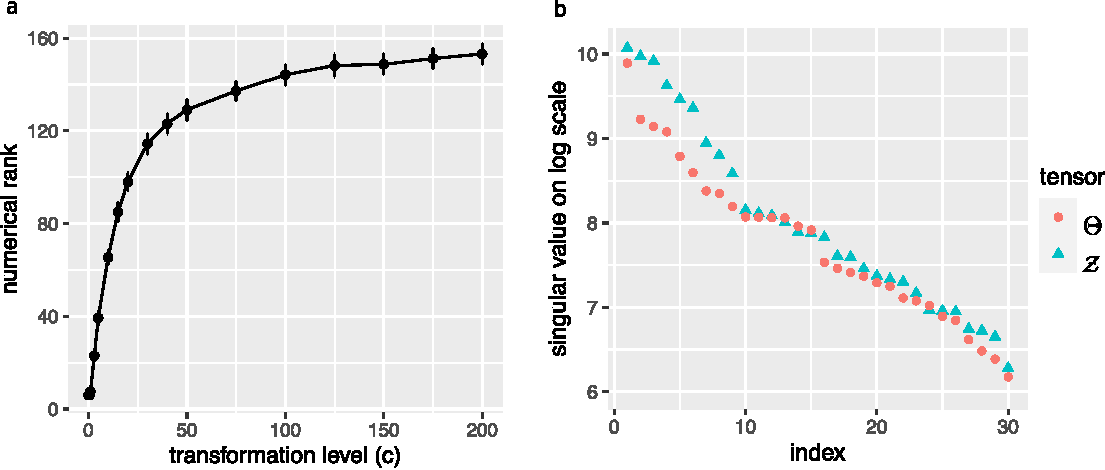
\includegraphics[width=0.78\textwidth]{figure/example_comb.pdf}
\caption{(a) Tensor rank vs.\ $c$ in the first example. (b) Top $d=30$ tensor singular values in the second example. }
\label{fig:example}
\end{figure}

The second example demonstrates the inadequacy of classical low-rankness in representing special structures. Here we consider the signal tensor of the form $\Theta=\log(1+\tZ)$, where $\tZ\in\mathbb{R}^{d\times d\times d}$ is an order-3 tensor with entries $\tZ(i,j,k)=d^{-1}\max(i,j,k)$ for $i,j,k\in\{1,\ldots,d\}$. The matrix analogy of $\Theta$ was studied in graphon analysis~\cite{chan2014consistent}. In this case neither $\Theta$ nor $\tZ$ is low-rank; in fact, the rank is no smaller than the dimension $d$ as illustrated in Figure~\ref{fig:example}b. Again, classical low-rank models fail to address this type of tensor structure. 

In the above and many other examples, the signal tensors $\Theta$ of interest have high rank. Classical low-rank models will miss these important structures. The observations have motivated us to develop more flexible tensor modeling. 


{\bf Our contributions.} We develop a new model called sign representable tensors to address the aforementioned challenges. 
Figure~\ref{fig:demo} illustrates our main idea. Our approach is built on the sign series representation of the signal tensor, and we propose to estimate the sign tensors through a series of weighted classifications. In contrast to existing methods, our method is guaranteed to recover a wide range of low- and high-rank signals. We highlight two main contributions that set our work apart from earlier literature. 

Statistically, the problem of high-rank tensor estimation is challenging. Existing estimation theory~\citep{anandkumar2014tensor,montanari2018spectral,cai2019nonconvex} exclusively focuses on the regime of fixed $r$ growing $d$. However, such premise fails in high-rank tensors, where the rank may grow with, or even exceed, the dimension. A proper notion of nonparametric complexity is crucial. We show that, somewhat surprisingly, the sign tensor series not only preserves all information in the original signals, but also brings the benefits of flexibility and accuracy over classical low-rank models. The results fill the gap between parametric (low-rank) and nonparametric (high-rank) tensors, thereby greatly enriching the tensor model literature. 

Computationally, a number of polynomial-time algorithms are readily available for 1-bit tensor estimation~\cite{wang2018learning, han2020optimal, ghadermarzy2018learning}. These algorithms enjoy computational efficiency while being restricted to binary inputs. Our work is orthogonal to these algorithm development, and we show that the high-rank tensor estimate is provably reducible to a series of binary tensor problems with carefully-designed weights. This reduction provides a generic engine to empower existing algorithms for a wider range of structured tensor problems. We use a divide-and-concur approach to combine efficient base algorithms, thereby achieving computational accuracy without the need to reinvent the wheel. The flexibility to import and adapt existing tensor algorithms is one advantage of our method. 

We also highlight the challenges associated with tensors compared to matrices. High-rank matrix estimation is recently studied under nonlinear models~\citep{ganti2015matrix} and subspace clustering~\citep{pmlr-v70-ongie17a,fan2019online}. However, high-rank tensor problems is more challenging, because the tensor rank often exceeds the dimension when order $K$ greater than two~\citep{anandkumar2017analyzing}. This is in sharp contrast to matrices ($K=2$). We show that, applying matrix methods to higher-order tensors results in suboptimal estimates. A full exploitation of the higher-order structure is needed; this is another challenge we address in this paper.

{\bf Notation.} We use $[n]=\{1,\ldots,n\}$ for $n$-set with $n\in\mathbb{N}_{+}$, $a_n\lesssim b_n$ if $\lim_{n\to\infty} a_n/b_n\leq c$ for some constant $c>0$, and $a_n\asymp b_n$ if $c_1\leq \lim_{n\to \infty} a_n/b_n\leq c_2$ for some constants $c_1,c_2>0$. We use $\tO(\cdot)$ to denote the big-O notation, $\tilde \tO(\cdot)$ the variant hiding logarithmic factors. Let $\Theta\in\mathbb{R}^{d_1\times \cdots \times d_K}$ denote an order-$K$ $(d_1,\ldots,d_K)$-dimensional tensor, and $\Theta(\omega)\in\mathbb{R}$ denote the tensor entry indexed by $\omega \in[d_1]\times \cdots \times [d_K]$. An event $A$ is said to occur ``with very high probability'' if $\mathbb{P}(A)$ tends to 1 faster than any polynomial of tensor dimension $d:=\min_k d_k \to\infty$. The tensor rank~\citep{hitchcock1927expression} is defined by $\text{rank}(\Theta)=\min\{r\in\mathbb{N}\colon \Theta=\sum_{s=1}^r\ma^{(1)}_s\otimes\cdots\otimes \ma^{(K)}_s\}$, where $\ma^{(k)}_s\in\mathbb{R}^{d_k}$ are vectors for $k\in[K], s\in[r]$, and $\otimes$ denotes the outer product of vectors. We use $\sign(\cdot)\colon \mathbb{R}\to\{-1,1\}$ to denote the sign function, where $\sign(y)=1$ if $y\geq 0$ and $-1$ otherwise. We allow univariate functions, such as $\sign(\cdot)$ and general $f\colon \mathbb{R}\to\mathbb{R}$, to be applied to tensors in an element-wise manner. 


\section{Model and proposal overview}\label{sec:overview}
Let $\tY$ be an order-$K$ $(d_1,\ldots,d_K)$-dimensional tensor generated from the model
\begin{equation}\label{eq:model}
\tY=\Theta+\tE,
\end{equation}
where $\Theta\in\mathbb{R}^{d_1\times \cdots \times d_K}$ is an unknown signal tensor, and $\tE$ is a noise tensor consisting of zero-mean, independent but not necessarily identically distributed entries. We allow heterogenous noise, in that the marginal distribution of noise entry $\tE(\omega)$ may depend on $\omega$. For a cleaner exposition, we assume the noise is bounded and the range of $Y$ is in $[-1,1]$; the extension to a sub-Gaussian noise is provided in Section~\ref{sec:subGaussian}. Our observation is an incomplete data tensor from~\eqref{eq:model}, denoted  $\tY_\Omega$, where $\Omega\subset[d_1]\times\cdots\times[d_K]$ is the index set of observed entries. We consider a general model on $\Omega$ that allows both uniform and non-uniform samplings. Specifically, let $\Pi=\{p_\omega\}$ be an arbitrarily predefined probability distribution over the full index set with $\sum_{\omega\in[d_1]\times \cdots \times [d_K]}p_\omega=1$. We use $\omega\sim \Pi$ to denote the sampling rule, meaning $\omega$ in $\Omega$ are i.i.d.\ draws with replacement from distribution $\Pi$. The goal is to estimate $\Theta$ from $Y_{\Omega}$. Note that $\Theta$ is not necessarily low-rank. 

{\bf Proposal intuition.} Before describing our main results, we provide the intuition behind our method. In the two examples in Section~\ref{sec:intro}, the high-rankness in the signal $\Theta$ makes the estimation challenging. Now let us examine the sign of the $\pi$-shifted signal $\sign(\Theta-\pi)$ for any given $\pi\in[-1,1]$. It turns out that, these sign tensors share the same sign patterns as low-rank tensors. Indeed, the signal tensor in the first example has the same sign pattern as a rank-$4$ tensor, since $\sign(\Theta-\pi)=\sign(\tZ-f^{-1}(\pi))$. The signal tensor in the second example has the same sign pattern as a rank-2 tensor, since $\sign(\Theta(i,j,k)-\pi)=\sign(\max(i,j,k)-d(e^{\pi}-1))$ (see Example~\ref{eq:example} in Section~\ref{sec:representation}).

The above observation suggests a general framework to estimate both low- and high-rank signal tensors. Figure~\ref{fig:demo} illustrates the main crux of our method. We propose to estimate the signal tensor $\Theta$ by taking the average over structured sign tensors
\begin{equation}\label{eq:intuition}
\hat \Theta = {1\over 2H+1}\sum_{\pi \in \tH} \sign(\hat \tZ_\pi), \ \text{where}\ \hat \tZ_\pi=\argmin_{\text{low rank tensor $\tZ$}} \text{Weighted-Loss}(\sign(\tZ), \sign (\tY_\Omega-\pi)).
\end{equation}
Here $\sign(\hat \tZ_\pi)\in\{-1,1\}^{d_1\times\cdots\times d_K}$ is the sign tensor estimated at a series of $\pi\in \tH=\{\small-1,\ldots,$ $-{1/H},0, {1/H},\ldots,1\}$, and Weighted-Loss$(\cdot,\cdot)$ denotes a classification objective function with an entry-specific weight to each tensor entry; its specific form will be described in Section~\ref{sec:identifiability}. To obtain $\sign(\hat \tZ_\pi)$ for a given $\pi$, we propose to dichotomize the data tensor into a sign tensor $\sign (\tY_\Omega-\pi)$ and estimate the de-noised sign by performing weighted classification. 

\begin{figure}[h!]
\captionsetup{font=footnotesize}
\centerline{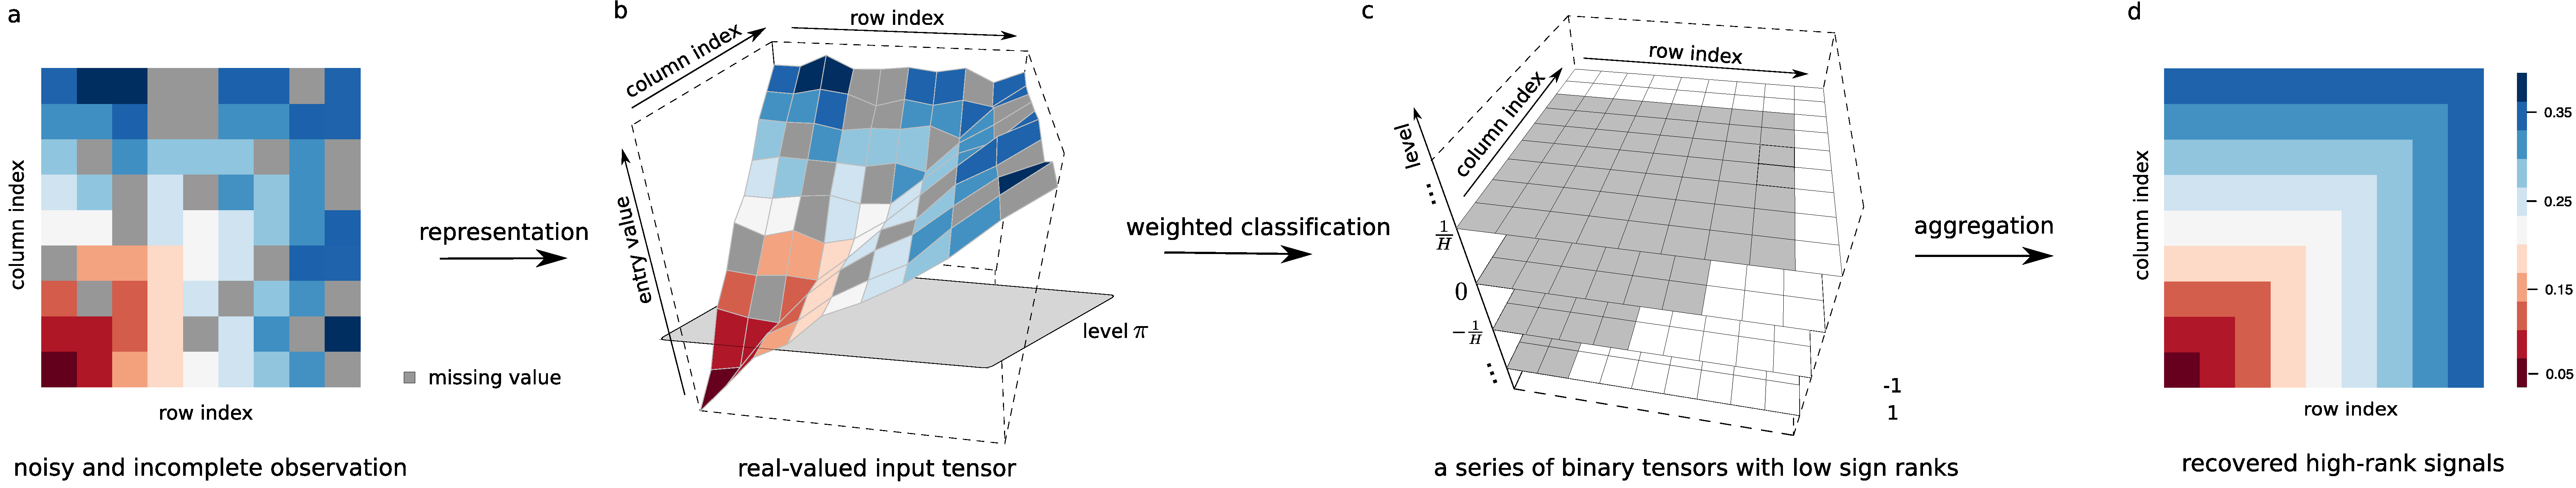
\includegraphics[width=1.05\textwidth]{figure/demo.pdf}}
\caption{Illustration of our method in the context of an order-2 tensor (a.k.a.\ matrix). (a): a noisy, incomplete tensor input. (b)-(c): Estimation of sign tensor series $\sign(\Theta-\pi)$ for $\pi\in  \{-1,\ldots,-{1/ H},0,{1/H},\ldots,1\}$. (d): recovered signal $\hat \Theta$. The depicted signal is a full-rank matrix based on Example~\ref{eq:example} in Section~\ref{sec:representation}.}\label{fig:demo}
\end{figure}

Our approach is built on the nonparametric sign representation of signal tensors. We show that a careful aggregation of dichotomized data not only preserves all information in the original signals, but also brings benefits of accuracy and flexibility over classical low-rank models. Unlike traditional methods, the sign representation is guaranteed to recover both low- and high-rank signals. In addition, a total of $H=\text{poly}(d)$ dichotomized problems suffice to recover $\Theta$ under the considered model.  The method therefore enjoys both statistical effectiveness and computational efficiency. 

\section{Oracle properties of sign representable tensors}\label{sec:representation}
This section develops sign representable tensor models for $\Theta$ in~\eqref{eq:model}. We characterize the algebraic and statistical properties of sign tensor series, which serves the foundation for our method. 

\subsection{Sign-rank and sign tensor series}\label{sec:sign-rank}
Let $\Theta$ be the tensor of interest, and $\sign (\Theta)$ the corresponding sign pattern. The sign patterns induce an equivalence relationship between tensors. Two tensors are called sign equivalent, denoted $\simeq$, if they have the same sign pattern.

\begin{defn}[Sign-rank]
The sign-rank of a tensor $\Theta\in\mathbb{R}^{d_1\times \cdots \times d_K}$ is defined by the minimal rank among all tensors that share the same sign pattern as $\Theta$; i.e.,
\[
\srank(\Theta) = \min \{\rank(\Theta')\colon  \Theta'\simeq \Theta,\ \Theta'\in\mathbb{R}^{d_1\times \cdots \times d_K}\}.
\]
\end{defn}
This concept is important in combinatorics~\citep{cohn2013fast}, complexity theory~\citep{alon2016sign}, and quantum mechanics~\citep{de2003nondeterministic}; we extend the notion to continuous-valued tensors. Note that the sign-rank concerns only the sign pattern but discards the magnitude information of $\Theta$. In particular, $\srank(\Theta)=\srank(\sign \Theta)$. 

Like most tensor problems~\citep{hillar2013most}, determining the sign-rank is NP hard in the worst case~\citep{alon2016sign}. Fortunately, tensors arisen in applications often possess special structures that facilitate analysis. The sign-rank is upper bounded by tensor rank. More generally, we show the following properties.
\begin{prop}[Upper bounds of the sign-rank]~\label{cor:monotonic} \hfill
\begin{enumerate}[label={2.\arabic*},wide, labelwidth=!, labelindent=0pt,itemsep=0ex,parsep=0ex,topsep=-7pt]
\item[(a)] [Upper bounds] For any strictly monotonic function $g\colon \mathbb{R}\to \mathbb{R}$ with $g(0)=0$,  we have $\textup{srank}(\Theta)\leq\rank(g(\Theta))$.
\item[(b)] [Broadness] For every order $K\geq 2$ and dimension $d$, there exist tensors $\Theta\in\mathbb{R}^{d\times \cdots \times d}$ such that $\rank(\Theta)\geq d$ but $\srank(\Theta-\pi)\leq 2$ for all $\pi\in\mathbb{R}$.  
\end{enumerate}
\end{prop}

Propositions~\ref{cor:monotonic} demonstrates the strict broadness of low sign-rank family over the usual low-rank family. 
In particular, the sign-rank can be much smaller than the tensor rank, as we have shown in the two examples of Section~\ref{sec:intro}. We provide several additional examples in Section~\ref{sec:high-rank} in which the tensor rank grows with dimension $d$ but the sign-rank remains a constant. The results highlight the advantages of using sign-rank in the high-dimensional tensor analysis. 

We now introduce a tensor family, which we coin as ``sign representable tensors''.
\begin{defn}[Sign representable tensors] 
Fix a level $\pi\in[-1,1]$. A tensor $\Theta$ is called $(r,\pi)$-sign representable, if the tensor $(\Theta-\pi)$ has sign-rank bounded by $r$. A tensor $\Theta$ is called $r$-sign (globally) representable, if $\Theta$ is $(r,\pi)$-sign representable for all $\pi\in[-1,1]$. The collection $\{\sign(\Theta-\pi)\colon \pi \in[-1,1]\}$ is called the sign tensor series. 
We use $\caliP(r)=\{\Theta\colon \max_{\pi\in[-1,1]}\srank(\Theta-\pi)\leq r\}$ to denote the $r$-sign representable tensor family.
\end{defn}

We next show that the $r$-sign representable tensor family is a general model that incorporates most existing tensor models, including low-rank tensors, single index models, GLM models, and structured tensors with repeating entries. 

\begin{example}[CP/Tucker low-rank models] The CP and Tucker low-rank tensors are the two most popular tensor models~\citep{kolda2009tensor}. Let $\Theta$ be a low-rank tensor with CP rank $r$. We see that $\Theta$ belongs to the sign representable family; i.e., $\Theta\in\caliP(r+1)$ (the constant $1$ is due to $\rank(\Theta-\pi)\leq r+1$). Similar results hold for Tucker low-rank tensors $\Theta\in\caliP(r+1)$, where $r=\prod_kr_k$ with $r_k$ being the $k$-th mode Tucker rank of $\Theta$.  
\end{example} 
\begin{example}[Tensor block models (TBMs)] Tensor block model~\citep{wang2019multiway,chi2020provable} assumes a checkerboard structure among tensor entries under marginal index permutation. The signal tensor $\Theta$ takes at most $r$ distinct values, where $r$ is the total number of multiway blocks. Our model incorporates TBM because $\Theta \in \caliP(r)$. 
\end{example}

\begin{example}[Generalized linear models (GLMs)] Let $\tY$ be a binary tensor from a logistic model~\citep{wang2018learning} with mean $\Theta=\text{logit}(\tZ)$, where $\tZ$ is a latent low-rank tensor. Notice that $\Theta$ itself may be high-rank (see Figure~\ref{fig:example}a). By definition, $\Theta$ is a low-rank sign representable tensor. Same conclusion holds for general exponential-family models with a (known) link function~\citep{hong2020generalized}. 
\end{example}

\begin{example}[Single index models (SIMs)] Single index model is a flexible semiparametric model proposed in economics~\citep{robinson1988root} and high-dimensional statistics~\citep{balabdaoui2019least,ganti2017learning}. The SIM assumes the existence of a (unknown) monotonic function $g\colon \mathbb{R}\to \mathbb{R}$ such that $g(\Theta)$ has rank $r$. We see that $\Theta$ belongs to the sign representable family; i.e., $\Theta\in \caliP(r+1)$. 
\end{example}

\begin{example}[Structured tensors with repeating entries]\label{eq:example} Here we revisit the model introduced in Figure~\ref{fig:example}b of Section~\ref{sec:intro}. Let $\Theta$ be an order-$K$ tensor with entries $\Theta(i_1,\ldots,i_K)=\log(1+\max_kx^{(k)}_{i_k})$, where $x^{(k)}_{i_k}$ are given numbers in $[0,1]$ for all $i_k\in[d_k], k\in[K]$. We conclude that $\Theta \in \caliP(2)$, because the sign tensor $\sign(\Theta-\pi)$ with an arbitrary $\pi\in(0,\ \log 2)$ is a block tensor with at most two blocks (see Figure~\ref{fig:demo}c). Similar results extend to structured tensors with entries $\Theta(i_1,\ldots,i_K)=g(\max_kx^{(k)}_{i_k})$, where $g(\cdot)$ is a polynomial of degree $r$. In this case, $\Theta$ is a high-rank tensor with at most $d_{\max}$ distinct entries but we have $\Theta\in \caliP(2r)$ (see proofs in Section~\ref{sec:high-rank}). 
\end{example}


\subsection{Statistical characterization of sign tensors via weighted classification}\label{sec:identifiability}
We now provide the explicit form of the weighted loss introduced in~\eqref{eq:intuition}, and show that sign tensors are characterized by weighted classification. The results bridge the algebraic and statistical properties of sign representable tensors.
 
For a given $\pi \in [-1,1]$, define a $\pi$-shifted data tensor $\bar \tY_\Omega$ with entries $\bar \tY(\omega) = (\tY(\omega)-\pi)$ for $\omega\in \Omega$. We propose a weighted classification objective function
\begin{equation}\label{eq:sample}
L(\tZ, \bar \tY_\Omega)= {1\over |\Omega|}\sum_{\omega \in \Omega}\ \KeepStyleUnderBrace{|\bar \tY(\omega)|}_{\text{weight}}\  \times \ \KeepStyleUnderBrace{| \sign \tZ(\omega)-\sign \bar \tY(\omega)|}_{\text{classification loss}},
\end{equation}
where $\tZ\in\mathbb{R}^{d_1\times \cdots \times d_K}$ is the decision variable to be optimized, $|\bar \tY(\omega)|$ is the entry-specific weight equal to the distance from the tensor entry to the target level $\pi$. The entry-specific weights incorporate the magnitude information into classification, where entries far away from the target level are penalized more heavily in the objective. In the special case of binary tensor $\tY\in\{-1,1\}^{d_1\times\cdots\times d_K}$ and target level $\pi=0$, the loss~\eqref{eq:sample} reduces to usual classification loss. 

Our proposed weighted classification function~\eqref{eq:sample} is important for characterizing $\sign(\Theta-\pi)$. Define the weighted classification risk 
\begin{equation}\label{eq:population}
\textup{Risk}(\tZ)=\mathbb{E}_{\tY_\Omega}L(\tZ,\bar\tY_\Omega),
\end{equation}
where the expectation is taken with respect to $\tY_\Omega$ under model~\eqref{eq:model} and the sampling distribution $\omega\sim\Pi$. %Note that
The form of $\textup{Risk}(\cdot)$ implicitly depends on $\pi$; we suppress $\pi$ when no confusion arises. 

\begin{prop}[Global optimum of weighted risk]\label{prop:global}
Suppose the data $\tY_\Omega$ is generated from model~\eqref{eq:model} with $\Theta \in \caliP(r)$. Then, for all $\bar \Theta$ that are sign equivalent to $\sign(\Theta-\pi)$, 
\begin{align}\label{eq:optimal}
\textup{Risk}(\bar \Theta )&=\inf\{\textup{Risk}(\tZ)\colon \tZ\in\mathbb{R}^{d_1\times \cdots \times d_K}\}
=\inf\{\textup{Risk}(\tZ)\colon \textup{rank} (\tZ)\leq r\}.
\end{align}
\end{prop}
The results show that the sign tensor $\sign(\Theta-\pi)$ optimizes the weighted classification risk. This fact suggests a practical procedure to estimate $\sign(\Theta-\pi)$ via empirical risk optimization of $L(\tZ,\bar \tY_\Omega)$. In order to establish the recovery guarantee, we shall address the uniqueness (up to sign equivalence) for the optimizer of $\risk(\cdot)$. The local behavior of $\Theta$ around $\pi$ plays a key role in the accuracy. 

Some additional notation is needed for stating the results in full generality. Let $d_\text{total}=\prod_{k=1}^K d_k$ denote the total number of tensor entries, and $\Delta s = 1/d_\text{total}$ a small tolerance. We quantify the distribution of tensor entries $\Theta(\omega)$ using a pseudo density, i.e., histogram with bin width $2\Delta s$. Let $G(\pi):=\mathbb{P}_{\omega\sim \Pi}[\Theta(\omega)\leq \pi]$ denote the cumulative distribution function (CDF) of $\Theta(\omega)$ under $\omega\sim \Pi$. We partition $[-1,1]=\tN^c \cup \tN$, such that the pseudo density based on $2\Delta$-bin is uniformly bounded over $\tN^c$; i.e,
\[
\tN^c=\left\{\pi\in[-1,1] \colon {G(\pi+{\Delta s})-G(\pi-{\Delta s})\over \Delta s} \leq C \right\},\ \text{for some universal constant $C>0$},
\]
and $\tN$ otherwise. Both $\Theta$ and its induced CDF $G$ implicitly depend on the tensor dimension. 

\begin{assumption}[$\alpha$-smoothness]\label{ass:margin} Fix $\pi \in\tN^c$. Assume there exist constants $\alpha=\alpha(\pi)> 0, c=c(\pi) >0$, independent of tensor dimension, such that, 
\begin{equation}\label{eq:smooth}
\sup_{\Delta s \leq t<\rho(\pi, \tN)}{G(\pi+{t})-G(\pi-{t})\over t^\alpha} \leq c,
\end{equation}
where $\rho(\pi,\tN):=\min_{\pi'\in \tN}|\pi-\pi'|+\Delta s$ denotes the adjusted distance from $\pi$ to the nearest point in $\tN$. The largest possible $\alpha=\alpha(\pi)$ in~\eqref{eq:smooth} is called the smoothness index at level $\pi$. We make the convention that $\alpha=\infty$ if the numerator in~\eqref{eq:smooth} is zero. A tensor $\Theta$ is called $\alpha$-globally smooth, if~\eqref{eq:smooth} holds with global constants $\alpha>0, c>0$ for all $\pi\in\tN^c$. 
\end{assumption}

The smoothness index $\alpha$ quantifies the intrinsic hardness of recovering $\sign(\Theta-\pi)$ from $\risk(\cdot)$. 
The value of $\alpha$ depends on both the sampling distribution $\omega\sim \Pi$ and the behavior of $\Theta(\omega)$. 
The recovery is easier at levels where points are less concentrated around $\pi$ with a large value of $\alpha>1$, or equivalently, when $G(\pi)$ remains almost  flat around $\pi$. A small value of $\alpha<1$ indicates the nonexistent (infinite) density at level $\pi$, or equivalently, when the $G(\pi)$ jumps by greater than the tolerance $\Delta s$ at $\pi$. Table~\ref{tab:simulation} illustrates the $G(\pi)$ for various models of $\Theta$ (see Section~\ref{sec:simulation}). 

We now reach the main theorem in this section. For two tensors $\Theta_1,\Theta_2$, define the mean absolute error (MAE) as
$\text{MAE}(\Theta_1, \Theta_2)=\mathbb{E}_{\omega\sim \Pi}|\Theta_1(\omega)-\Theta_2(\omega)|.$

\begin{thm}[Identifiability]\label{thm:population}Assume $\Theta\in\caliP(r)$ is $\alpha$-globally smooth. Then, for all $\pi\in \tN^c$ and tensors $\bar \Theta \simeq \sign(\Theta-\pi)$, we have
\[
\textup{MAE}(\sign \tZ, \sign \bar \Theta) \lesssim C(\pi)\left[\textup{Risk}(\tZ)-\textup{Risk}( \bar \Theta)\right]^{\alpha/(\alpha+1)}+\Delta s, \quad \text{for all }\tZ\in\mathbb{R}^{d_1\times \cdots \times d_K},
\]
where $C(\pi)>0$ is independent of $\tZ$. 
\end{thm}
The result establishes the recovery stability of sign tensors $\sign (\Theta-\pi)$ using optimization with population risk~\eqref{eq:population}. The bound immediately shows the uniqueness of the optimizer for $\text{Risk}(\cdot)$ up to a  $\Delta s$-measure set under $\Pi$. We find that a higher value of $\alpha$ implies more stable recovery, as intuition would suggest. Similar results hold for optimization with sample risk~\eqref{eq:sample} (see Section~\ref{sec:estimation}). 

We conclude this section by applying Assumption~\ref{ass:margin} to the examples described in Section~\ref{sec:sign-rank}. For simplicity, suppose $\Pi$ is the uniform sampling. 
The tensor block model is $\infty$-globally smooth. This is because the set $\tN$ consists of finite $2\Delta s$-bin's covering the distinct block means in $\Theta$. Furthermore, we have $\alpha= \infty$ for all $\pi \in \tN^c$, since the numerator in~\eqref{eq:smooth} is zero. Similarly, the high-rank $(d,d,d)$-dimensional tensor $\Theta(i,j,k) = \log(1+{1\over d}\max(i,j,k))$ is $\infty$-globally smooth because $\alpha=\infty$ for all $\pi$ except those in $\tN$, where $\tN$ collects $d$ many $2\Delta s$-bin's covering $\log(1+i/d)$ for all $i \in[d]$.


\section{Nonparametric tensor completion via sign series}\label{sec:estimation}

In previous sections we have established the sign series representation and its relationship to classification. In this section, we present our learning reduction proposal in details (Figure~\ref{fig:demo}). We provide the estimation error bound and address the empirical implementation of the method. 


\subsection{Statistical error and sample complexity}\label{sec:error}
Given a noisy incomplete tensor observation $\tY_\Omega$ from model~\eqref{eq:model}, we cast the problem of estimating $\Theta$ into a series of weighted classifications. Specifically, we propose the signal tensor estimate using averaged structured sign tensors
\begin{equation}\label{eq:est}
\hat \Theta = {1\over 2H+1}\sum_{\pi \in \tH}\sign{\hat \tZ_\pi}, \quad \text{with}\quad \hat \tZ_\pi = \argmin_{\tZ\colon \text{rank}\tZ\leq r} L(\tZ, \tY_\Omega-\pi),
\end{equation}
where $\tH=\{-1,\ldots,-{1/ H}, 0, {1/H},\ldots,1\}$ is the series of levels to aggregate, $L(\cdot,\cdot)$ denotes the weighted classification objective defined in~\eqref{eq:sample}, and the rank constraint on $\tZ$ follows from Proposition~\ref{prop:global}. For the theory, we assume the true $r$ is known; in practice, $r$ could be chosen in a data adaptive fashion via cross-validation or elbow method~\citep{hastie2009elements}. 

The next theorem establishes the statistical convergence for the sign tensor estimate~\eqref{eq:est}.

\begin{thm}[Sign tensor estimation]\label{thm:classification} Suppose $\Theta\in\caliP(r)$ and $\Theta(\omega)$ is $\alpha$-globally smooth under $\omega\sim \Pi$. Let $\hat \tZ_\pi$ be the estimate in~\eqref{eq:est}, $d=\max_{k\in[K]}d_k$, and $t_d ={dr\log|\Omega|\over |\Omega|}\lesssim 1$. Then, for all $\pi\in\tN^c$, with very high probability over $\tY_\Omega$, 
\begin{align}\label{eq:bound}
\textup{MAE}(\sign \hat \tZ_\pi, \sign(\Theta-\pi)) \lesssim t_d^{\alpha/( \alpha+2)}+{1 \over \rho^2(\pi, \tN)}t_d.
\end{align}
\end{thm}
Theorem~\ref{thm:classification} provides the error bound for the sign tensor estimation. Compared to the population results in Theorem~\ref{thm:population}, we explicitly reveal the dependence of accuracy on the sample complexity and the level $\pi$. The result demonstrates the polynomial decay of sign errors with $|\Omega|$.  Our sign estimate achieves consistent recovery using as few as $\tilde \tO(dr)$ noisy entries. 

Recall that $\tN$ collects the levels for which the sign tensor is possibly nonrecoverable. Let $|\tN|$ be the covering number of $\tN$ with $2\Delta s$-bin's, i.e, $|\tN| = \lceil \text{Leb}(\tN)/2\Delta s \rceil$, where $\text{Leb}(\cdot)$ is the Lebesgue measure and $\lceil \cdot \rceil$ is the ceiling function. Combining the sign representability of the signal tensor and the sign estimation accuracy, we obtain our main results on nonparametric tensor estimation. 

\begin{thm}[Tensor estimation error]\label{thm:estimation} Consider the same conditions of Theorem~\ref{thm:classification}. Let $\hat \Theta$ be the estimate in~\eqref{eq:est}. For any resolution parameter $H\in\mathbb{N}_{+}$, with very high probability over $\tY_\Omega$,
\begin{equation}\label{eq:bound2}
\textup{MAE}(\hat \Theta, \Theta)\lesssim (t_d\log H)^{\alpha\over \alpha+2}+{1+|\tN|\over H}+{t_dH\log H}.
\end{equation}
In particular, setting $\footnotesize H= (1+|\tN|)^{1/2} t_d^{-1/2}\asymp \text{poly}(d)$ yields the tightest upper bound in~\eqref{eq:bound2}.
\end{thm}

Theorem~\ref{thm:estimation} demonstrates the convergence rate of our tensor estimation. The bound~\eqref{eq:bound2} reveals three sources of errors: the estimation error for sign tensors, the bias from sign series representations, and the variance thereof. The resolution parameter $H$ controls the bias-variance tradeoff. We remark that the signal estimation error~\eqref{eq:bound2} is generally no better than the corresponding sign error~\eqref{eq:bound}. This is to be expected, since magnitude estimation is  a harder problem than sign estimation. 

In the special case of full observation with equal dimension $d_1=\cdots=d_K=d$ and bounded $|\tN|\leq C$, our signal estimate achieves convergence
\begin{equation}
\textup{MAE}(\hat \Theta, \Theta)\lesssim rd^{-(K-1)\min({\alpha\over \alpha+2},\ {1\over 2})}\log^2 d,
\end{equation}
by setting $H\asymp d^{(K-1)/2}$. Compared to earlier methods, our estimation accuracy applies to both low- and high-rank signal tensors. The rate depends on the sign complexity $\Theta\in\caliP(r)$, and this $r$ is often much smaller than the usual tensor rank (see Section~\ref{sec:sign-rank}). Our result also reveals that the convergence becomes favorable as the order of data tensor increases. 

We apply our method to the main examples in Section~\ref{sec:sign-rank}, and compare the results with existing literature. The numerical comparison is provided in Section~\ref{sec:simulation}. 

\begin{customexample}{2}[TBMs]
Consider a tensor block model with $r$ multiway blocks. Our result implies a rate $\tilde \tO(d^{-(K-1)/2})$ by taking $\alpha=\infty$ and $|\tN| \leq r^K\lesssim \tO(1)$. This rate agrees with the  previous root-mean-square error (RMSE) for block tensor estimation~\citep{wang2019multiway}.
\end{customexample}

\begin{customexample}{3} [GLMs] 
Consider a GLM tensor $\Theta=g(\tZ)$, where $g$ is a known link function and $\tZ$ is a latent low-rank tensor. Suppose the CDF of $\Theta(\omega)$ is uniformly bounded as $d\to\infty$. Applying our results with $\alpha=1$ and finite $|\tN|$ yields $\tilde \tO(d^{-(K-1)/3})$. This rate is slightly slower than the parametric RMSE rate~\citep{zhang2018tensor,wang2018learning}, as expected. The reason is that our estimate remains valid for unknown $g$ and general high-rank tensors. The nonparametric rate is the price one has to pay for not knowing the form $\Theta=g(\tZ)$ as a priori. 
\end{customexample}

\begin{customexample}{4}[SIMs]
The earlier example has shown the nonparametric rate $\tilde \tO(d^{-(K-1)/3})$ when applying our method to single index tensor model. In the matrix case with $K=2$, our result yields error rate $\tilde \tO(d^{-1/3})$, which is faster than the RMSE rate $\tO(d^{-1/4})$ obtained by \cite{ganti2015matrix}. 
\end{customexample}

\begin{customexample}{5}[Structured tensors with repeating entries]
We consider a more general model than that in Section~\ref{sec:intro}. Consider a $r$-sign representable tensor $\Theta\in \caliP(r)$ with at most $d$ distinct entries with repetition pattern. Applying our results with $\alpha=\infty$ and $|\tN|=d$ yields the rate $\tilde \tO(d^{-(K-2)/2})$. 
\end{customexample}

The following corollary reveal the sample complexity for nonparamtric tensor completion. 
\begin{cor}[Sample complexity for nonparametric completion] Assume the same conditions of Theorem~\ref{thm:estimation} and bounded $|\tN|$. Then, with high probability over $\tY_\Omega$, 
\[
\textup{MAE}(\hat \Theta, \Theta)\to 0, \quad \text{as}\quad {|\Omega|\over {dr} \log^2 |\Omega|}\to \infty.
\]
\end{cor}
Our result improves earlier work~\citep{yuan2016tensor,ghadermarzy2019near,pmlr-v119-lee20i} by allowing both low- and high-rank signals. Interestingly, the sample requirements depend only on the sign complexity $dr$ but not the nonparametric complexity $\alpha$. Note that $\tilde \tO(dr)$ roughly matches the degree of freedom of sign tensors, suggesting the optimality of our sample requirements. 



\subsection{Implementation via learning reduction}
This section addresses the practical implementation of our estimation~\eqref{eq:est}. We take a learning reduction approach by dividing the full procedure into a meta algorithm and $2H+1$ base algorithms. The meta algorithm takes the average of $(2H+1)\asymp \text{poly}(d)$ sign tensors, whereas each base algorithm estimates the tensor $\sign(\Theta-\pi)$ given binary input $\sign(\tY-\pi)$ and a target rank $r$. The full procedure is described in Algorithm~\ref{alg:tensorT} and Figure~\ref{fig:demo}.


\begin{algorithm}[h!]
  \caption{Nonparametric tensor completion via learning reduction}\label{alg:tensorT}
 \begin{algorithmic}[1] 
\INPUT Noisy and incomplete data tensor $\tY_\Omega$, rank $r$, resolution parameter $H$, ridge penalty $\lambda$.
\For {$\pi \in \tH=\{ -1, \ldots, -{1\over H}, 0, {1\over H},\ldots, 1\}$}
\State Define $\pi$-shifted tensor $\bar \tY=\tY-\pi$ and corresponding sign tensor $\sign(\bar \tY)=\sign(\tY-\pi)$. 
\State Perform 1-bit tensor estimation algorithm~\citep{ghadermarzy2018learning,wang2018learning,hong2020generalized,alquier2019estimation} on $\bar \tY_\Omega$ and obtain 
\begin{align}\hat \tZ_\pi\leftarrow \argmin_{\text{low-rank }\tZ}\sum_{\omega\in \Omega} |\bar \tY(\omega)|F(\tZ(\omega)\sign\bar \tY(\omega))+\lambda\FnormSize{}{\tZ}^2,
\end{align} where $F(\cdot)$ is the large-margin loss and $\lambda$ is the penalty parameter.
\EndFor
\OUTPUT Estimated signal tensor $\hat \Theta_F={1\over 2H+1}\sum_{\pi \in \tH}\sign(\hat \tZ_\pi)$.
\end{algorithmic}
\end{algorithm}

The base algorithm reduces to a low-rank 1-bit tensor estimation problem. Following the common practice in classification~\cite{bartlett2006convexity}, we replace the 0-1 loss $\ell(z,y)=|\sign z - \sign y|$ in~\eqref{eq:sample} with a continuous large-margin loss $F(m)$ where $m=z\sign(y)$ is the margin. Examples of large-margin loss are hinge loss $F(m) = (1-m)_+$, logistic loss $F(m) =\log(1+e^{-m})$, and $\psi$-loss $F(m)=2\min(1,(1-m)_+)$ with $m_{+}=\max(m,0)$. A number of polynomial-time algorithms with convergence guarantees are readily available for this problem~\citep{ghadermarzy2018learning,wang2018learning,hong2020generalized,alquier2019estimation}. We implement hinge loss~\citep{alquier2019estimation,genzel2020robust,he2017kernelized} which maintains desirable statistical properties as in 0-1 loss,
Here $\risk_F(\cdot)$ is defined similarly as in~\eqref{eq:population} with hinge loss in place of 0-1 loss. 



\begin{assumption}[Assumptions on surrogate loss]\label{ass:loss} \hfill
\begin{enumerate}
\item[(a)] (Approximation error) For any given $\pi\in[-1,1]$, assume there exist a sequence of tensors $\tZ^{(n)}_\pi\in\caliP(r)
$, such that $\risk_F(\tZ^{(n)}_\pi)-\risk_F(\bar\Theta)\leq a_n$, for some sequence $a_n\to 0$ as $n\to\infty$. Furthermore, assume $\FnormSize{}{\tZ_{\pi}^{(n)}} \leq J$ for some constant $J>0$. 
\item[(b)]  $F(z)=(1-z)_{+}$ is hinge loss.
\end{enumerate}
\end{assumption}

\noindent
Assumption~\ref{ass:loss}(a) quantifies the representation capability of and $\caliP(r)$.  Assumption~\ref{ass:loss}(b) implies the Fisher consistency bound for the weighted risk \citep{scott2011surrogate},
\begin{equation*} \label{eq:fisher}
\risk(\tZ)-\risk(\Theta-\pi)\lesssim \risk_{F}(\tZ)-\risk_{F}(\Theta-\pi), \text{ for all $\pi\in[-1,1]$ and all $\tZ$}.
\end{equation*}
The Fisher consistency enable us to relate the excess risk of the large margin loss to that of 0-1 loss. Under Assumption \ref{ass:loss},  the resulting estimate from Algorithm~\ref{alg:tensorT} enjoys both statistical and computational efficiency. 

\begin{thm}[Large-margin estimation]~\label{thm:extension} 
Consider the same setup as in Theorem~\ref{thm:estimation}, and denote $ t_n={d_{\max}rK\log n \over n}$. Suppose the surrogate loss $F$ satisfies Assumption~\ref{ass:loss} with $a_n \lesssim t_n^{(\alpha+1)/(\alpha+2)}$. Set $\lambda\asymp t_n^{(\alpha+1)/(\alpha+2)}+t_n/\rho(\pi,\tN)$ in \eqref{eq:largemgopt}. Then, with high probability at least $1-\exp(-nt_n)$,  we have:
\begin{enumerate}[label=(\alph*)]
\item (Sign tensor estimation). For all $\pi\in[-1,1]$ except for a finite number of levels,
\begin{equation}\label{eq:sfe}
\textup{MAE}(\sign(\hat \tZ_\pi,\sign(\Theta-\pi)) \lesssim t_n ^{\alpha\over 2+\alpha}+{1\over \rho^2(\pi,\tN)}t_n.
\end{equation}

\item (Tensor estimation). 
\begin{equation}\label{eq:rfs}
\textup{MAE}(\hat\Theta_F,\Theta) \lesssim  \left(t_n\log H\right)^{\alpha \over 2+\alpha}+\frac{1+|\tN|}{H}+t_nH\log H.
\end{equation}
In particualr, setting $H\asymp(1+|\tN|)^{1/2} t_n^{-1/2}$ yields the tightest upper bound in~\eqref{eq:rfs}.
\end{enumerate}
\end{thm}

In principle, uses can choose their own favorite large-margin losses, as long as the base algorithms are sample efficient. The comparison between various large-margin losses has been studied before~\cite{bartlett2006convexity}. Note that, instead of using $\hat \tZ_\pi$ as in existing 1-bit tensor algorithms~\cite{ghadermarzy2018learning,wang2018learning}, we use $\sign(\hat \tZ_\pi)$ for more challenging nonparametric estimation. The sign aggregation brings the benefits of flexibility and accuracy over classical low-rank models. 


\section{Simulations}\label{sec:simulation}
In this section, we compare our nonparametric tensor method ({\bf NonParaT}) with two alternative approaches: low-rank tensor CP decomposition ({\bf CPT}), and the matrix version of our method applied to tensor unfolding ({\bf NonParaM}). We assess the performance under both complete and incomplete observations. The signal tensors are generated based on four models listed in Table~\ref{tab:simulation}. The simulation covers a wide range of complexity, including block tensors, transformed low rank tensors, min/max hypergraphon with logarithm and exponential functions. We consider order-3  tensors of equal dimension $d_1=d_2=d_3=d$, and set $d\in \{15, 20,\ldots,55,60\}$, $r=2$, $H=10+{(d-15)/ 5}$ in Algorithm~\ref{alg:tensorT}. For {\bf NonParaM}, we apply Algorithm~\ref{alg:tensorT} to each of the three unfolded matrices and report the average error. All summary statistics are averaged across $30$ replicates.  

\begin{table*}[h]
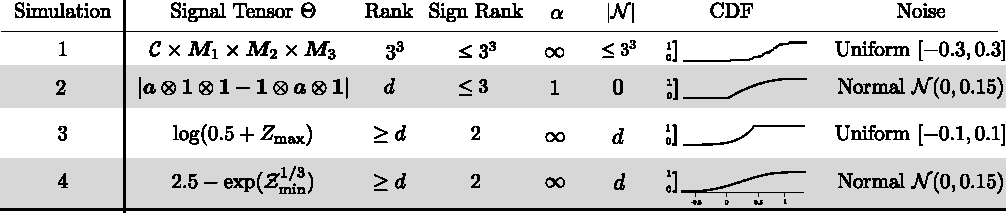
\includegraphics[width=1\textwidth]{figure/simulation.pdf}
\caption{Simulation models used for comparison. We use $\mM_k\in\{0,1\}^{d\times 3}$ to denote membership matrices, $\tC\in\mathbb{R}^{3\times 3\times 3}$ the block means, $\ma={1\over d}(1,2,\ldots,d)^T \in\mathbb{R}^d$, $\tZ_{\max}$ and $\tZ_{\min}$ are order-3 tensors with entries ${1\over d}\max(i,j,k)$ and ${1\over d}\min(i,j,k)$, respectively.}\label{tab:simulation}
\end{table*}


Figure~\ref{fig:compare1} compares the estimation error under full observation. The MAE decreases with tensor dimension for all three methods. We find that our method {\bf NonParaT} achieves the best performance in all scenarios, whereas the second best method is {\bf CPT} for models 1-2, and {\bf NonParaM} for models 3-4. One possible reason is that models 1-2 have controlled multilinear tensor rank, which makes tensor methods {\bf NonParaT} and {\bf CPT} more accurate than matrix methods. For models 3-4, the rank exceeds the tensor dimension, and therefore, the two nonparametric methods {\bf NonParaT} and {\bf NonparaM} exhibit the greater advantage for signal recovery. 



Figure~\ref{fig:compare2} shows the completion error against observation fraction. We fix $d=40$ and gradually increase the observation fraction ${|\Omega|\over d^3}$ from 0.3 to 1. We find that {\bf NonParaT} achieves the lowest error among all methods. Our simulation covers a reasonable range of  complexities; for example, model 1 has $3^3$ jumps in the CDF of signal $\Theta$, and models 2 and 4 have unbounded noise. Nevertheless, our method shows good performance in spite of model misspecification. This robustness is appealing in practice because the structure of underlying signal tensor is often unknown. 

\begin{figure}[h!]
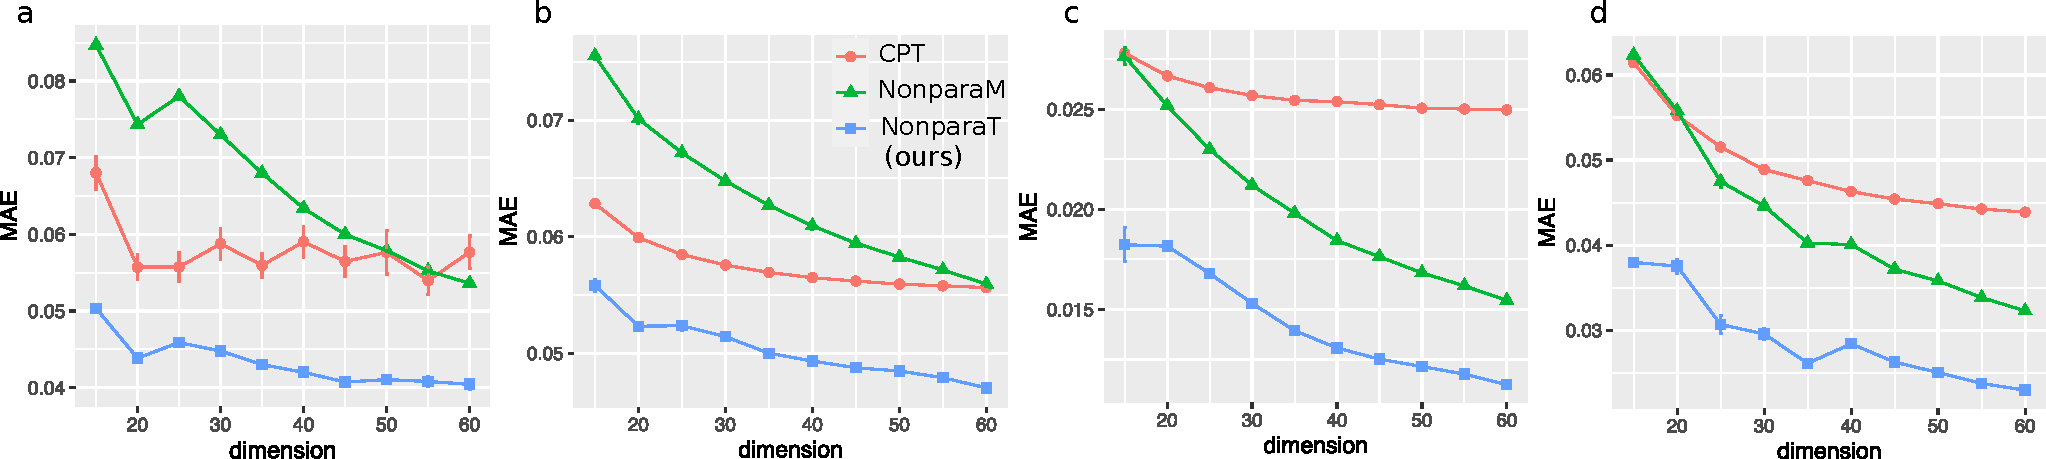
\includegraphics[width=\textwidth]{figure/fig1-4v2.pdf}
\caption{Estimation error versus tensor dimension. Panels (a)-(d) correspond to simulation models 1-4 in Table~\ref{tab:simulation}.}\label{fig:compare1}
\end{figure}


\begin{figure}[h!]
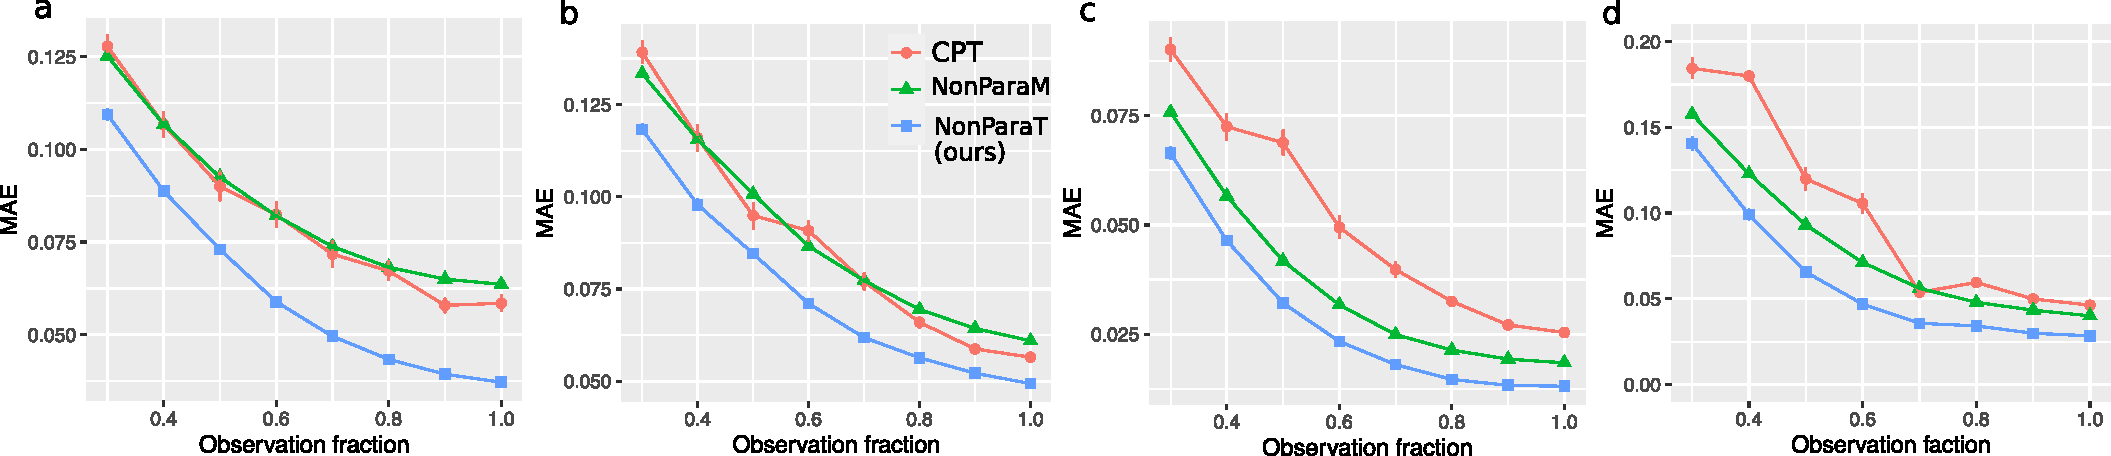
\includegraphics[width=\textwidth]{figure/fig5-8v2.pdf}
\caption{Completion error versus observation fraction. Panels (a)-(d) correspond to simulation models 1-4 in Table~\ref{tab:simulation}. }\label{fig:compare2}
\end{figure}

\section{Data applications}
We apply our method to two tensor datasets, the MRN-114 human brain connectivity data~\citep{wang2017bayesian}, and NIPS word occurrence data~\citep{globerson2007euclidean}. 

\subsection{Brain connectivity analysis}
The brain dataset records the structural connectivity among 68 brain regions for 114 individuals along with their Intelligence Quotient (IQ) scores. We organize the connectivity data into an order-3 tensor, where entries encode the presence or absence of fiber connections between brain regions across individuals. 

\begin{figure}[h!]
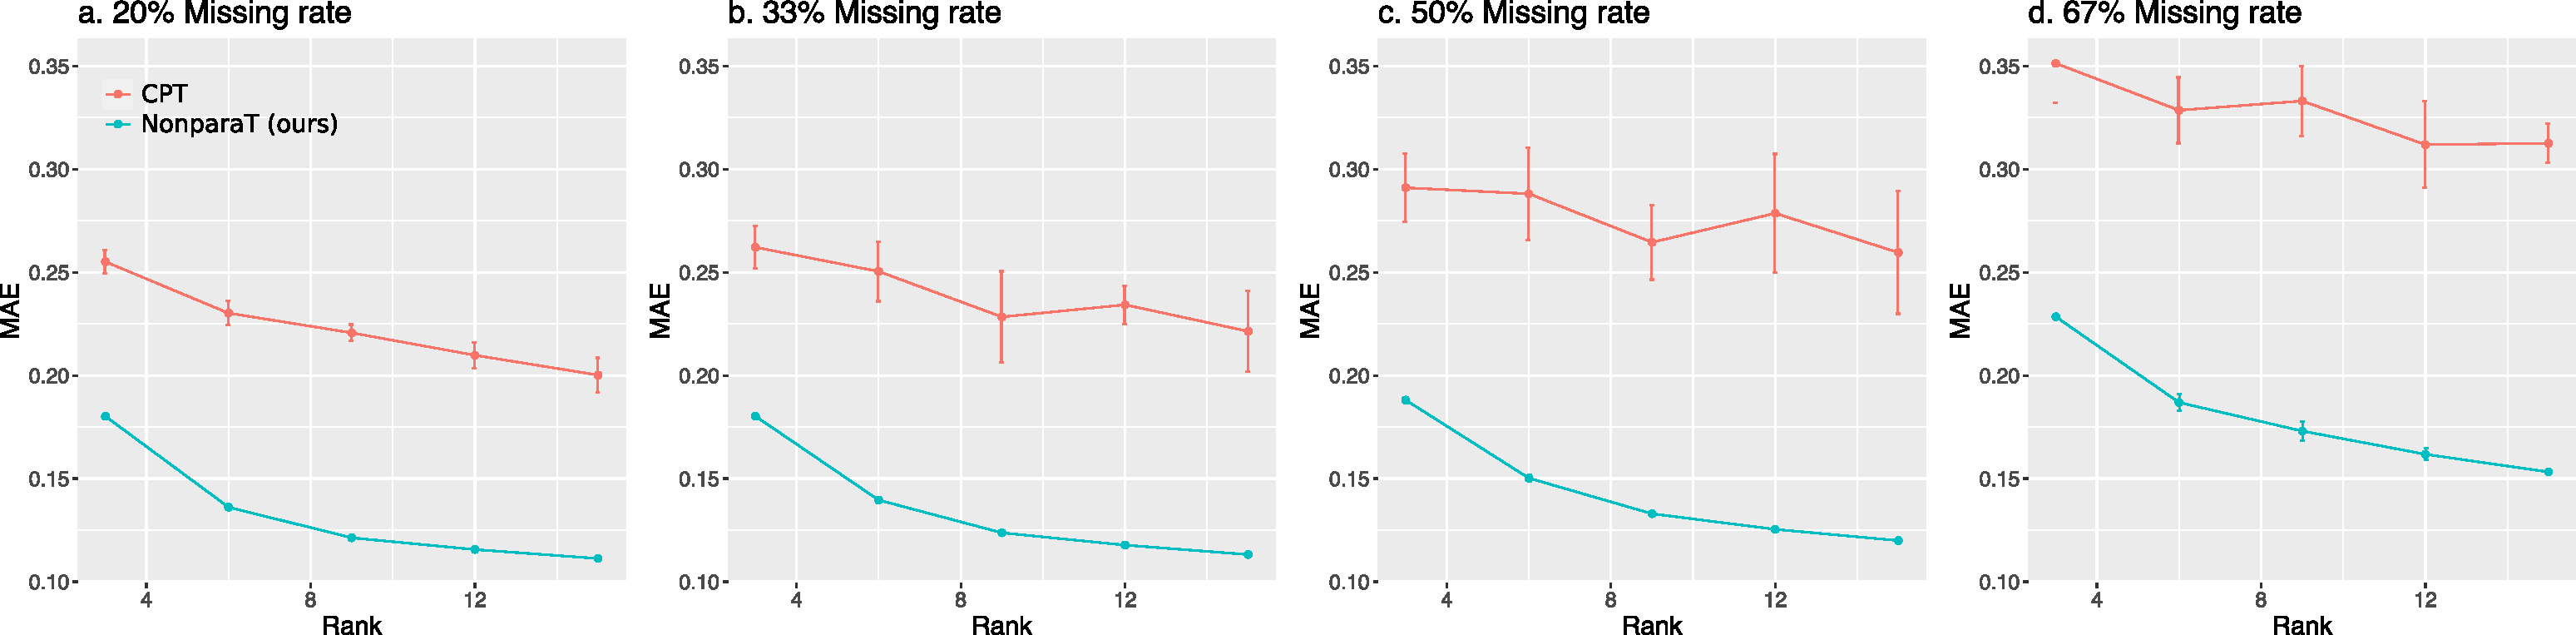
\includegraphics[width = \textwidth]{figure/brain_sim.pdf}
\caption{Estimation error versus rank under different missing rate. Panels (a)-(d) correspond to missing rate 20\%, 33\%, 50\%, and 67\%, respectively. Error bar represents the standard error over 5-fold cross-validations.}\label{fig:braincv}
\end{figure}

Figure~\ref{fig:braincv} shows the MAE based on 5-fold cross-validations with $r = 3,6,\ldots, 15$ and $H = 20$. We find that our method outperforms CPT in all combinations of ranks and missing rates. The achieved error reduction appears to be more profound as the missing rate increases. This trend highlights the applicability of our method in tensor completion tasks. In addition, our method exhibits a smaller standard error in cross-validation experiments as shown in Figure~\ref{fig:braincv} and Table~\ref{tab:data}, demonstrating the stability over CPT.  One possible reason is that that our estimate is guaranteed to be in $[0,1]$ (for binary tensor problem where $\tY\in\{0,1\}^{d_1\times\cdots d_K}$) whereas CPT estimation may fall outside the valid range $[0,1]$. 


\begin{table}[h!]
\centering
\resizebox{1\textwidth}{!}{
\begin{tabular}{c|c|c|c|c|c}
\Xhline{2\arrayrulewidth}
\multicolumn{6}{c}{MRN-114 brain connectivity dataset}\\
\Xhline{2\arrayrulewidth}
Method             &$r =3$        & $r=6$ &  $r=9$&$r=12$&$r = 15$\\
\hline
NonparaT (Ours)& ${\bf 0.18}(0.001)$ &$ {\bf 0.14}(0.001)$ & ${\bf 0.12}(0.001)$&${\bf 0.12}(0.001)$&${\bf 0.11}(0.001)$\\
Low-rank CPT &$0.26(0.006)$ & $0.23(0.006$)&$0.22(0.004)$&$0.21(0.006)$&$0.20(0.008)$\\
 \Xhline{2\arrayrulewidth}
 \multicolumn{6}{c}{NIPS word occurrence dataset}\\
 \Xhline{2\arrayrulewidth}
Method             &$r =3$        & $r=6$ &  $r=9$&$r=12$&$r = 15$\\
\hline
NonparaT (Ours) & ${\bf 0.18}(0.002)$ & ${\bf 0.16}(0.002)$ & ${\bf 0.15}(0.001)$& ${\bf 0.14}(0.001)$&${\bf 0.13}(0.001)$\\
 \hline
Low-rank CPT &$0.22(0.004)$ & $0.20(0.007)$ & $0.19(0.007)$&$0.17(0.007)$&$0.17(0.007)$\\
  \hline
Naive imputation (Baseline)& \multicolumn{5}{c}{$0.32(.001)$}
\end{tabular}
}
\caption{MAE comparison in the brain data and NIPS data analysis. Reported MAEs are averaged over five runs of cross-validation, with 20\% entries for testing and 80\% for training, with standard errors in parentheses. Bold numbers indicate the minimal MAE among three methods. For low-rank CPT, we use R function {\tt rTensor} with default hyperparameters, and for our method, we set $H=20$.}\label{tab:data}
\end{table}

We next investigate the pattern in the estimated signal tensor. Figure~\ref{fig:signal}a shows the identified top edges associated with IQ scores. Specifically, we first obtain a denoised tensor $\hat \Theta\in\mathbb{R}^{68\times 68\times 114}$ using our method with $r=10$ and $H=20$. Then, we perform a regression analysis of $\hat \Theta(i,j,\colon)\in\mathbb{R}^{144}$ against the normalized IQ score across the 144 individuals. The regression model is repeated for each edge $(i,j)\in[68]\times[68]$. We find that top edges represent the interhemispheric connections in the frontal lobes.  The result is consistent with recent research on brain connectivity with intelligence~\citep{li2009brain,wang2017bayesian}.



\subsection{NIPS data analysis}

The NIPS dataset consists of word occurrence counts in papers published from 1987 to 2003. We focus on the top 100 authors, 200 most frequent words, and normalize each word count by log transformation with pseudo-count 1. The resulting dataset is an order-3 tensor with entry representing the log counts of words by authors across years. 


Table~\ref{tab:data} compares the prediction accuracy of different methods. We find that our method substantially outperforms the low-rank CP method for every configuration under consideration. Further increment of rank appears to have little effect on the performance. 
The comparison highlights the advantage of our method in achieving accuracy while maintaining low complexity. In addition, we also perform naive imputation where the missing values are predicted using the sample average. Both our method and CPT outperform the naive imputation, implying the necessity of incorporating tensor structure in the analysis.

\begin{figure}[h!]
\centering
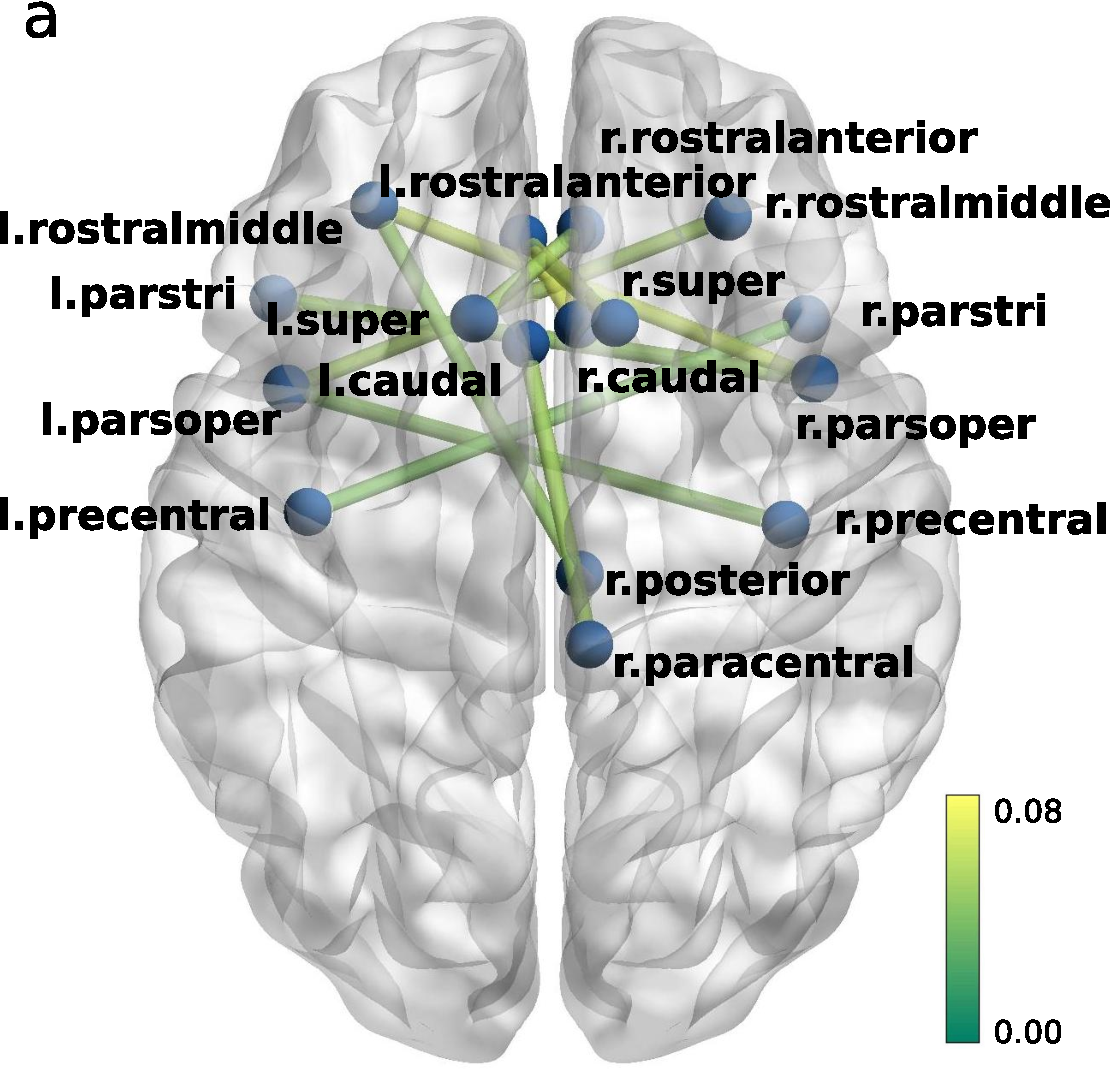
\includegraphics[width=.39\textwidth]{figure/brainIQ.pdf}
\hspace{1cm}
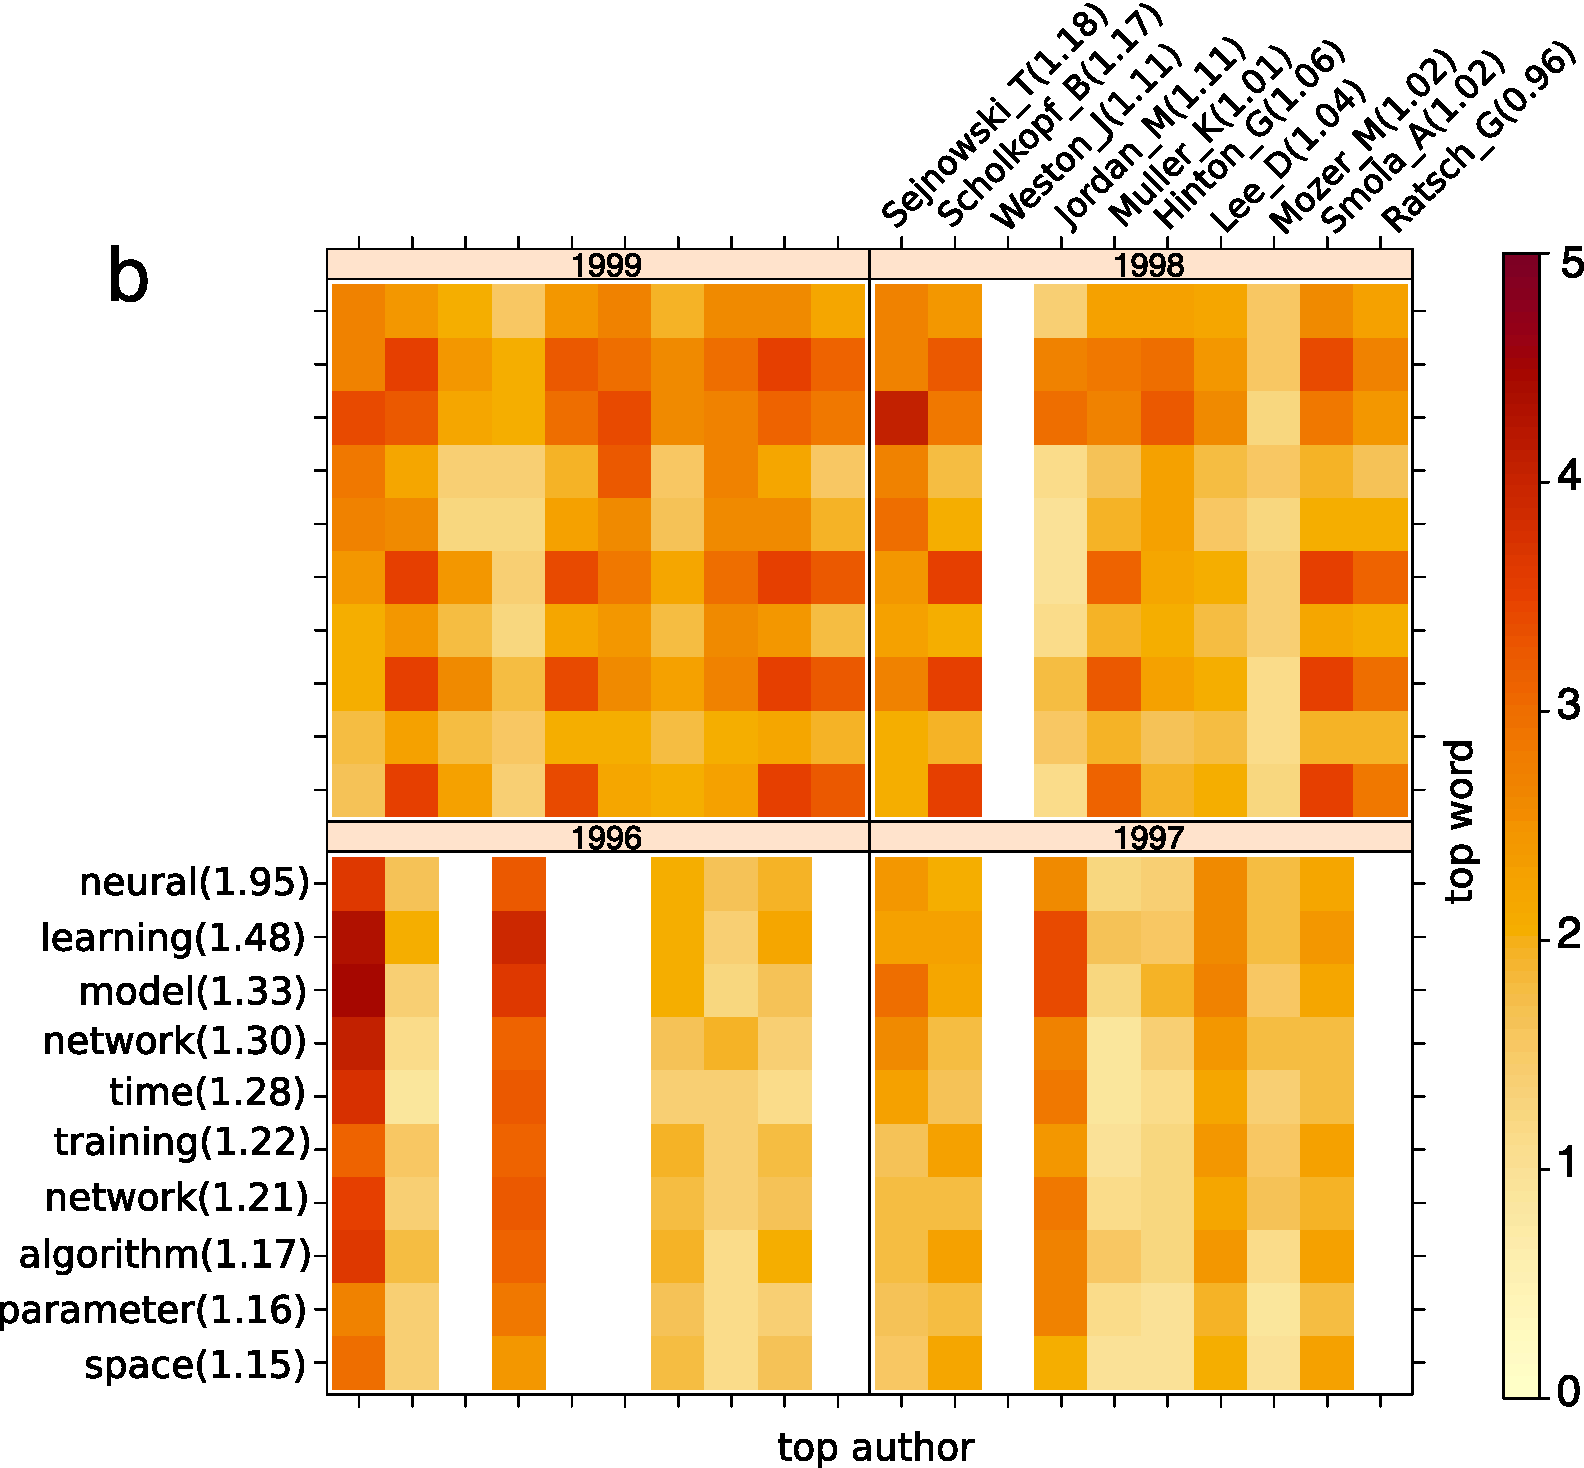
\includegraphics[width=.495\textwidth]{figure/signal.pdf}
\caption{Estimated signal tensors in the data analysis. (a) top edges associated with IQ scores in the brain connectivity data. The color indicates the estimated IQ effect size. (b) top authors and words for years 1996-1999 in the NIPS data. Authors and words are ranked by marginal averages based on $\hat \Theta$, where the marginal average is denoted in the parentheses.
}\label{fig:signal}
\end{figure}


We next examine the estimated signal tensor $\hat \Theta$ from our method.  Figure~\ref{fig:signal}b illustrates the results from NIPS data, where we plot the entries in $\hat \Theta$ corresponding to top authors and most-frequent words (after excluding generic words such as \emph{figure}, \emph{results}, etc). The identified pattern is consistent with the active topics in the NIPS publication. Among the top words are \emph{neural} (marginal mean = 1.95), \emph{learning} (1.48), and \emph{network} (1.21), whereas top authors are \emph{T.\ Sejnowski} (1.18), \emph{B.~Scholkopf} (1.17), \emph{M.\ Jordan} (1.11), and \emph{G.\ Hinton} (1.06). We also find strong heterogeneity among word occurrences across authors and years. For example, \emph{training} and \emph{algorithm} are popular words for \emph{B.\ Scholkopf} and \emph{A.\ Smola} in 1998-1999, whereas \emph{model} occurs more often in \emph{M.\ Jordan} and in 1996. The detected pattern and achieved accuracy demonstrate the applicability of our method.

\section{Additional results and proofs}
In this section, we provides additional results not covered in previous sections. Section~\ref{sec:numericalrank} gives detailed explanation to the examples mentioned in Section~\ref{sec:intro}. Section~\ref{sec:high-rank} supplements Section~\ref{sec:sign-rank} by providing more theoretical results on sign rank and its relationship to tensor rank. Section~\ref{sec:proofs} collects the proofs for theorems in the main texts.  Lastly,  Section~\ref{sec:subGaussian} extends all  results to unbounded observations with sub-Gaussian noise.

\subsection{Sensitivity of tensor rank to monotonic transformations}\label{sec:numericalrank}
In Section~\ref{sec:intro} of the main paper, we have provided a motivating example to show the sensitivity of tensor rank to monotonic transformations. Here, we describe the details of the example set-up. 

The step 1 is to generate a rank-3 tensor $\tZ$ based on the CP representation
\[
\tZ=\ma^{\otimes 3}+\mb^{\otimes 3}+\mc^{\otimes 3},
\]
where $\ma,\mb,\mc\in\mathbb{R}^{30}$ are vectors consisting of $N(0,1)$ entries, and the shorthand $\ma^{\otimes 3}=\ma\otimes \ma\otimes \ma$ denotes the Kronecker power. We then apply $f(z)=(1+\exp(-cz))^{-1}$ to $\tZ$ entrywise, and obtain a transformed tensor $\Theta=f(\tZ)$. 

The step 2 is to determine the rank of $\Theta$. Unlike matrices, the exact rank determination for tensors is NP hard. Therefore, we choose to compute the numerical rank of $\Theta$ as an approximation.  The numerical rank is determined as the minimal rank for which the relative approximation error is below $0.1$, i.e.,
\begin{equation}\label{eq:numeric}
 \hat r(\Theta)=\min\left\{s\in\mathbb{N}_{+}\colon \min_{\hat \Theta\colon \rank(\hat \Theta)\leq s}{\FnormSize{}{\Theta-\hat \Theta}\over \FnormSize{}{\Theta}} \leq 0.1\right\}.
\end{equation}
We compute $\hat r(\Theta)$ by searching over $s\in\{1,\ldots,30^2\}$, where for each $s$, we (approximately) solve the least-square minimization using CP function in R package {\tt rTensor}. 
We repeat steps 1-2 ten times, and plot the averaged numerical rank of $\Theta$ versus transformation level $c$ in Figure~\ref{fig:example}a.  

\subsection{Tensor rank and sign-rank}\label{sec:high-rank}
In the main paper, we have provided several tensor examples with high tensor rank but low sign-rank. This section provides more examples and their proofs. 
Unless otherwise specified, let $\Theta$ be an order-$K$ $(d,\ldots,d)$-dimensional tensor. 
\begin{example}[Structured tensors with repeating entries]\label{example:max} Suppose the tensor $\Theta$ takes the form 
\[
\Theta(i_1,\ldots,i_K)=\log\left(1+{1\over d}\max(i_1,\ldots,i_K)\right), \ \text{for all }(i_1,\ldots,i_K)\in[d]^K.
\]
 Then 
 \[
 \rank(\Theta)\geq d, \quad \text{and}\quad \srank(\Theta-\pi)\leq 2\ \text{for all }\pi\in\mathbb{R}. 
 \]
\end{example}
\begin{proof}[Proof of Example~\ref{example:max}]
We first prove the results for $K=2$. The full-rankness of $\Theta$ is verified from elementary row operations as follows
\begin{align}
\begin{pmatrix}
(\Theta_2-\Theta_1)/(\log(1+\frac{2}{d})-\log(1+\frac{1}{d}))\\(\Theta_3-\Theta_2)/(\log(1+\frac{3}{d})-\log(1+\frac{2}{d}))\\\vdots\\ (\Theta_d-\Theta_{d-1})/(\log(1+\frac{d}{d})-\log(1+\frac{d-1}{d}))\\\Theta_d/\log(1+\frac{d}{d})
\end{pmatrix} = \begin{pmatrix}
 1&          0  &      \ddots  &        \ddots       &          0 \\
1& 1 & \ddots &            \ddots   &   \ddots          \\
      \vdots &     \vdots & \ddots &       \ddots &    \ddots         \\
 1 & 1 &1 & 1 &0\\
 1 & 1 &1 & 1 &1
\end{pmatrix},
\end{align}
where $\Theta_i$ denotes the $i$-th row of $\Theta$. 
Now it suffices to show $\srank(\Theta-\pi)\leq 2$ for $\pi$ in the feasible range $(\log(1+{1\over d}),\ \log 2)$. In this case, there exists an index $i^*\in\{2,\ldots,d\}$, such that $\log(1+{i^*-1\over d})< \pi\leq \log(1+{i^*\over d})$. By definition, the sign matrix $\sign (\Theta-\pi)$ takes the form
\begin{equation}\label{eq:matrix}
\sign (\Theta(i,j)-\pi)=
\begin{cases}
-1, & \text{both $i$ and $j$ are smaller than $i^*$};\\
1, & \text{otherwise}.
\end{cases}
\end{equation}
Therefore, the matrix $\sign (\Theta-\pi)$ is a rank-2 block matrix, which implies $\srank(\Theta-\pi)=2$. 

We now extend the results to $K\geq 3$. By definition of the tensor rank, the rank of a tensor is lower bounded by the rank of its matrix slice.  So we have $\rank(\Theta)\geq \rank(\Theta(\colon,\colon,1,\ldots,1))=d$. For the sign rank with feasible $\pi$, notice that the sign tensor $\sign(\Theta-\pi)$ takes the similar form as in~\eqref{eq:matrix},
\begin{equation}\label{eq:entrywise}
\sign (\Theta(i_1,\ldots,i_K)-\pi)=
\begin{cases}
-1, & \text{$i_k<i^*$ for all $k\in[K]$};\\
1, & \text{otherwise},
\end{cases}
\end{equation}
where $i^*$ denotes the index that satisfies $\log(1+\frac{i^*-1}{d})<\pi\leq \log(1+\frac{i^*}{d})$.
The equation~\eqref{eq:entrywise} implies that $\sign(\Theta-\pi)=-2\ma^{\otimes K}+1$, where $\ma=(1,\ldots,1,0,\ldots,0)^T$ takes 1 on the $i$-th entry if $i<i^*$ and 0 otherwise. Henceforth $\srank(\Theta-\pi)=2$. 
\end{proof}

In fact, Example~\ref{example:max} is a special case of the following proposition. 

\begin{prop}[Structured tensors with repeating entries]\label{prop:repeat}Let $g\colon \mathbb{R}\to \mathbb{R}$ be a continuous function such that $g(z)=0$ has at most $r\geq 1$ distinct real roots. For given numbers $x^{(k)}_{i_k}\in[0,1]$ for all $i_k\in[d_k]$, define a tensor $\Theta\in\mathbb{R}^{d_1\times\cdots \times d_K}$ with entries 
\begin{equation}\label{eq:max}
\Theta(i_1,\ldots,i_K)=g(\max(x^{(1)}_{i_1},\ldots,x^{(K)}_{i_K})),\quad (i_1,\ldots,i_K)\in[d_1]\times\cdots\times[d_K].
\end{equation}
Then, the sign rank of $(\Theta-\pi)$ satisfies
\[
\srank(\Theta-\pi)\leq 2r.
\]
The same conclusion holds if we use $\min$ in place of $\max$ in~\eqref{eq:max}. 
\end{prop}
\begin{proof}[Proof of Proposition~\ref{prop:repeat}]
We reorder the tensor indices along each mode such that $x^{(k)}_{1}\leq \cdots \leq x^{(k)}_{d_k}$ for all $k\in[K]$. Based on the construction of $\tZ_{\max}$, the reordering does not change the rank of $\tZ_{\max}$ or $(\Theta-\pi)$. Let $z_1<\cdots<z_r$ be the $r$ distinct real roots for the equation $g(z)=\pi$. We separate the proof for two cases, $r=1$ and $r\geq 2$. 

\begin{itemize}[leftmargin=*,topsep=0pt,itemsep=-1ex,partopsep=1ex,parsep=1ex]
\item When $r=1$. The continuity of $g(\cdot)$ implies that the function $(g(z)-\pi)$ has at most one sign change point. Using similar proof as in Example~\ref{example:max}, we have
\begin{align}
&\sign(\Theta-\pi)=1-2\ma^{(1)}\otimes\cdots\otimes \ma^{(K)}\quad \text{ or } \quad \sign(\Theta-\pi) = 2\ma^{(1)}\otimes\cdots\otimes \ma^{(K)} -1,
\end{align}
where $\ma^{(k)}$ are binary vectors defined by
\[
\ma^{(k)}=(\KeepStyleUnderBrace{1,\ldots,1,}_{\text{positions for which $x_{i_k}^{k}<z_1$}}0,\ldots,0)^T, \quad \text{for }k\in[K].
\]
Therefore, $\srank(\Theta-\pi)\leq \rank(\sign(\Theta-\pi)) = 2$. 

\item When $r\geq 2$.   By continuity, the function $(g(z)-\pi)$ is non-zero and remains an unchanged sign in each of the intervals $(z_s, z_{s+1})$ for $1\leq s\leq r-1$. Define the index set 
\[
\tI=\{s\in\mathbb{N}_{+}\colon \text{the interval $(z_s, z_{s+1})$ in which $g(z)<\pi$}\}.
\] 
We now prove that the sign tensor $\sign(\Theta-\pi)$ has rank bounded by $2r-1$. To see this, consider the tensor indices for which $\sign(\Theta-\pi)=-1$,
\begin{align}\label{eq:support}
\{\omega\colon \Theta(\omega)-\pi <0 \} & = \{\omega \colon g(\tZ_{\max}(\omega))<\pi\} \notag \\
&=\cup_{s\in \tI} \{\omega\colon \tZ_{\max}(\omega)\in(z_s,z_{s+1})\}\notag\\
&=\cup_{s\in \tI}\Big( \{\omega\colon \text{$x^{(k)}_{i_k}< z_{s+1}$ for all $k\in[K]$}\}\cap \{\omega\colon \text{$x^{(k)}_{i_k}\leq z_{s}$ for all $k\in[K]$}\}^c\Big).
\end{align}
The equation~\eqref{eq:support} is equivalent to 
\begin{align}\label{eq:indicator}
\mathds{1}(\Theta(i_1,\ldots,i_K)< \pi)&
=\sum_{s\in \tI}\left( \prod_k \mathds{1}(x^{(k)}_{i_k}< z_{s+1}) - \prod_k \mathds{1}(x^{(k)}_{i_k}\leq z_{s})\right),
\end{align}
for all $(i_1,\ldots,i_K)\in[d_1]\times \cdots\times[d_K]$, where $\mathds{1}(\cdot)\in\{0,1\}$ denotes the indicator function. The equation~\eqref{eq:indicator} implies the low-rank representation of $\sign(\Theta-\pi)$,
\begin{equation}\label{eq:sum}
\sign(\Theta-\pi)=1-2\sum_{s\in \tI } \left(\ma^{(1)}_{s+1}\otimes\cdots\otimes \ma^{(K)}_{s+1} - \bar \ma^{(1)}_s\otimes\cdots\otimes \bar \ma^{(K)}_s\right),
\end{equation}
where $\ma^{(k)}_{s+1}, \ma^{(k)}_{s}$ are binary vectors defined by
\[
\ma^{(k)}_{s+1}=(\KeepStyleUnderBrace{1,\ldots,1,}_{\text{positions for which $x_{i_k}^{(k)}<z_{s+1}$}}0,\ldots, 0)^T,\quad \text{and}\quad
\bar \ma^{(k)}_s=(\KeepStyleUnderBrace{1,\ldots,1,}_{\text{positions for which $x_{i_k}^{(k)}\leq z_{s}$}}0,\ldots, 0)^T.
\]
Therefore, by~\eqref{eq:sum} and the assumption $|\tI|\leq r-1$, we conclude that 
\[
\srank(\Theta-\pi)\leq 1+2(r-1)=2r-1.
\]
\end{itemize}
Combining two cases yields that $\srank(\Theta-\pi)\leq 2r$ for any $r\geq 1$.
\end{proof}

We next provide several additional examples such that $\rank(\Theta)\geq d$ whereas $\srank(\Theta)\leq c$ for a constant $c$ independent of $d$. We state the examples in the matrix case, i.e, $K=2$. Similar conclusion extends to $K\geq 3$, by the following proposition. 
\begin{prop}[Rank relationship between matrices and tensors]\label{prop:connection}Let $\mM\in\mathbb{R}^{d_1\times d_2}$ be a matrix. For any given $K\geq 3$, define an order-$K$ tensor $\Theta\in\mathbb{R}^{d_1\times \cdots \times d_K}$ by
\[
\Theta=\mM\otimes \mathbf{1}_{d_3}\otimes \cdots \otimes \mathbf{1}_{d_K},
\] 
where $\mathbf{1}_{d_k}\in\mathbb{R}^{d_k}$ denotes an all-one vector, for $3\leq k\leq K$. Then we have
\[
\rank(\Theta)=\rank(\mM),\quad \text{and}\quad \srank(\Theta-\pi)=\srank(\mM-\pi) \ \text{for all $\pi\in\mathbb{R}$}.
\] 
\end{prop}
\begin{proof}[Proof of Proposition~\ref{prop:connection}]
The conclusion directly follows from the definition of tensor rank. 
\end{proof}

\begin{example}[Stacked banded matrices]\label{example:banded} Let $\ma=(1,2,\ldots,d)^T$ be a $d$-dimensional vector, and define a $d$-by-$d$ banded matrix $\mM=|\ma\otimes \mathbf{1}-\mathbf{1}\otimes \ma|$. Then
\[
\rank(\mM)=d,\quad \text{and}\quad \srank(\mM-\pi)\leq 3, \quad \text{for all }\pi\in \mathbb{R}.
\]
\end{example}
\begin{proof}[Proof of Example~\ref{example:banded}]
Note that $\mM$ is a banded matrix with entries
\[
\mM(i,j)={|i-j|}, \quad \text{for all }(i,j)\in[d]^2.
\]
Elementary row operation shows that $\mM$ is full rank as follows,
\begin{align}
\begin{pmatrix}
(\mM_1+\mM_d)/(d-1)\\
\mM_1-\mM_2\\
\mM_2-\mM_3\\
\vdots\\
\mM_{d-1}-\mM_{d}
\end{pmatrix} = 
\begin{pmatrix}
1&1&1&\cdots&1&1\\
-1&1&1&\cdots&1&1\\
-1&-1&1&\cdots&1&1\\
\vdots & \vdots & \vdots & \vdots & \vdots & \vdots\\
-1&-1&-1&\cdots&-1&1
\end{pmatrix}.
\end{align}

We now show $\srank(\mM-\pi)\leq 3$ by construction. Define two vectors $\mb=(2^{-1},2^{-2},\ldots,2^{-d})^T\in\mathbb{R}^d$ and $\text{rev}(\mb)=(2^{-d},\ldots,2^{-1})^T\in\mathbb{R}^d$. We construct the following matrix
\begin{equation}\label{eq:A}
\mA=\mb\otimes\text{rev}(\mb)+\text{rev}(\mb)\otimes\mb.
\end{equation}
The matrix $\mA\in\mathbb{R}^{d\times d}$ is banded with entries
\[
\mA(i,j)=\mA(j,i)=\mA(d-i,d-j)=\mA(d-j,d-i)=2^{-d-1}\left(2^{j-i}+2^{i-j}\right),\ \text{for all }(i,j)\in[d]^2.
\] 
Furthermore, the entry value $\mA(i,j)$ decreases with respect to $|i-j|$; i.e., 
\begin{equation}\label{eq:decrease}
\mA(i,j) \geq \mA(i',j'), \quad \text{for all }|i-j|\geq |i'-j'|.
\end{equation}
Notice that for a given $\pi\in\mathbb{R}$, there exists $\pi'\in\mathbb{R}$ such that $\sign(\mA-\pi')=\sign(\mM-\pi)$. This is because both $\mA$ and $\mM$ are banded matrices satisfying monotonicity~\eqref{eq:decrease}. By definition~\eqref{eq:A}, $\mA$ is a rank-2 matrix. Henceforce, $\srank(\mM-\pi)=\srank(\mA-\pi')\leq 3.$
\end{proof}

\begin{rmk} The tensor analogy of banded matrices $\Theta=|\ma\otimes\mathbf{1}\otimes \mathbf{1}-\mathbf{1}\otimes\ma\otimes \mathbf{1}|$ is used as simulation model 3 in the main paper.  
\end{rmk}

\begin{example}[Stacked identity matrices]\label{ex:identity}
Let $\mI$ be a $d$-by-$d$ identity matrix. Then
\[
\rank(\mI)=d,\quad\text{and}\quad  \srank(\mI-\pi)\leq 3 \ \text{for all }\pi\in\mathbb{R}.
\]
\end{example}
\begin{proof}[Proof of Proposition~\ref{ex:identity}]
Depending on the value of $\pi$, the sign matrix $\sign(\mI-\pi)$ falls into one of the two cases: 
\begin{enumerate}
\item[(a)] $\sign(\mI-\pi)$ is a matrix of all $1$, or of all $-1$; 
\item[(b)] $\sign(\mI-\pi)=2\mI-\mathbf{1}_d\otimes \mathbf{1}_d$.
\end{enumerate}
The first cases are trivial, so it suffices to show $\srank(\mI-\pi)\leq 3$ in the third case.   


Based on Example~\ref{example:banded}, the rank-2 matrix $\mA$ in~\eqref{eq:A} satisfies 
\[
\mA(i,j)
\begin{cases}
=2^{-d}, & i=j,\\
\geq 2^{-d}+2^{-d-2}, & i\neq j.
\end{cases}
\]
Therefore, $\sign\left(2^{-d}+2^{-d-3}-\mA\right)=2\mI-\mathbf{1}_d\otimes \mathbf{1}_d$. We conclude that $\srank(\mI-\pi)\leq \rank(2^{-d}+2^{-d-3}-\mA)=3$. 
\end{proof}

\subsection{Proofs}\label{sec:proofs}
\subsubsection{Proofs of Propositions~\ref{cor:monotonic}-\ref{prop:global}}
\begin{proof}[Proof of Proposition~\ref{cor:monotonic}] \hfill
\begin{enumerate}[label={2.\arabic*},wide, labelindent=0pt]
\item[Part (a).] The strictly monotonicity of $g$ implies that the inverse function $g^{-1}\colon \mathbb{R}\to \mathbb{R}$ is well-defined. 
When $g$ is strictly increasing, the mapping $x\mapsto g(x)$ is sign preserving. Specifically, if $x\geq 0$, then $g(x)\geq g(0)=0$. Conversely, if $g(x)\geq 0=g(0)$, then applying $g^{-1}$ to both sides gives $x\geq 0$.
When $g$ is strictly decreasing, the mapping $x\mapsto g(x)$ is sign reversing. Specifically, if $x\geq 0$, then $g(x)\leq g(0)=0$. Conversely, if $g(x)\geq 0=g(0)$, then applying $g^{-1}$ to both sides gives $x\leq 0$.
 Therefore, $\Theta\simeq g(\Theta)$,  or $\Theta\simeq -g(\Theta)$. Since constant multiplication  does not change the tensor rank,  we have $\srank(\Theta)=\srank(g(\Theta))\leq \rank (g(\Theta))$. 
\item[Part (b).] See Section~\ref{sec:high-rank} for constructive examples.
\end{enumerate}
\end{proof}

\begin{proof}[Proof of Proposition~\ref{prop:global}]
Fix $\pi\in[-1,1]$. Based on the definition of classification loss $L(\cdot,\cdot)$, the function $\risk(\cdot)$ relies only on the sign pattern of the tensor. Therefore, without loss of generality, we assume both $\bar \Theta, \tZ \in\{-1,1\}^{d_1\times \cdots \times d_K}$ are binary tensors. 
We evaluate the excess risk 
\begin{equation}\label{eq:risk}
\risk(\tZ)- \risk(\bar \Theta) = \mathbb{E}_{\omega\sim \Pi}\KeepStyleUnderBrace{\mathbb{E}_{\tY(\omega)}\left\{|\tY(\omega)-\pi|\left[\left|\tZ(\omega)-\sign(\bar \tY(\omega)) \right|-\left|\bar\Theta(\omega)-\sign(\bar \tY(\omega))\right|\right]\right\}}_{\stackrel{\text{def}}{=}I(\omega)}.
\end{equation}
Denote $y=\tY(\omega)$, $z=\tZ(\omega)$, $\bar \theta=\bar\Theta(\omega)$, and $\theta=\Theta(\omega)$. The expression of $I(\omega)$ is simplified as
\begin{align}\label{eq:I}
I(\omega)&= \mathbb{E}_{y|\omega}\left[ (y-\pi)(\bar \theta-z)\mathds{1}(y\geq \pi)+(\pi-y)(z-\bar \theta)\mathds{1}(y< \pi)\right]\notag \\
&= \mathbb{E}_{y|\omega}\left[(\bar \theta-z) (y-\pi)\right]\notag \\
&=  \left[\sign(\theta-\pi)-z\right]\left(\theta-\pi\right)\notag \\
&= |\sign(\theta-\pi)-z||\theta-\pi|\geq 0,
\end{align}
where the third line uses the fact $\mathbb{E}y=\theta$ and $\bar \theta=\sign(\theta-\pi)$, and the last line uses the assumption $z \in\{-1,1\}$. The equality~\eqref{eq:I} is attained when $z=\sign(\theta-\pi)$ or $\theta=\pi$. Combining~\eqref{eq:I} with~\eqref{eq:risk}, we conclude that, for all $\tZ\in\{-1,1\}^{d_1\times \cdots \times d_K}$, 
\begin{equation}\label{eq:minimum}
\risk(\tZ)- \risk(\bar \Theta) = \mathbb{E}_{\omega\sim \Pi} |\sign(\Theta(\omega)-\pi)-\tZ(\omega)||\Theta(\omega)-\pi|\geq 0.
\end{equation}
In particular, setting $\tZ=\bar \Theta=\sign(\Theta-\pi)$ in~\eqref{eq:minimum} yields the minimum. Therefore, 
\[
\risk(\bar \Theta)=\min\{\risk(\tZ)\colon \tZ\in \mathbb{R}^{d_1\times \cdots \times d_K}\} \leq \min\{\risk(\tZ)\colon \rank(\tZ)\leq r\}.
\]
Since $\srank(\Theta-\pi)\leq r$ by assumption, the last inequality becomes equality. The proof is complete. 
\end{proof}

\subsubsection{Proof of Theorem~\ref{thm:population}}
\begin{proof}[Proof of Theorem~\ref{thm:population}]
Fix $\pi\notin\tN$. Based on~\eqref{eq:minimum} in Proposition~\ref{prop:global}, we have
\begin{equation}\label{eq:population2}
\risk(\tZ)- \risk(\bar \Theta) = \mathbb{E}\left[|\sign \tZ-\sign\bar \Theta||\bar \Theta|\right].
\end{equation}
The Assumption~\ref{ass:margin} states that
\begin{align}\label{eq:ass}
\mathbb{P}\left(|\bar \Theta | \leq t\right) \leq 
\begin{cases}ct^\alpha, & \text{for all } \Delta s \leq t< \rho(\pi,\tN),\\
C\Delta s, & \text{for all }0\leq t< \Delta s.
\end{cases}
\end{align}
Without further specification, all relevant probability statements, such as $\mathbb{E}$ and $\mathbb{P}$, are with respect to $\omega\sim \Pi$. 

We divide the proof into two cases: $\alpha >0$ and $\alpha = \infty$.
\begin{itemize}[leftmargin=*,topsep=0pt,itemsep=-1ex,partopsep=1ex,parsep=1ex]
\item Case 1: $\alpha>0$. 

By~\eqref{eq:population2}, for all $0 \leq t< \rho(\pi, \tN)$,
\begin{align}\label{eq:1}
\risk(\tZ)- \risk(\bar \Theta) &\geq t\mathbb{E}\left(|\sign \tZ- \sign \bar\Theta|\mathds{1}\{|\bar\Theta|>t\}\right)
\notag \\
&\geq 2t\mathbb{P}\left(\sign\tZ \neq \sign \bar \Theta\text{ and }|\bar \Theta|>t   \right)\notag \\
& \geq 2t\Big\{\mathbb{P}\left(\sign\tZ \neq \sign \bar \Theta \right) - \mathbb{P}\left(|\bar \Theta|\leq t\right)\Big\}\notag\\
&\geq t\Big\{\textup{MAE}(\sign \tZ, \sign \bar \Theta) - C\Delta s - 2ct^\alpha \Big\},
\end{align}
where the last line follows from the definition of MAE and~\eqref{eq:ass}. We maximize the lower bound~\eqref{eq:1} with respect to $t$, and obtain the optimal $t_{\text{opt}}$,
\[
t_{\text{opt}}=\begin{cases}
\rho(\pi, \tN), & \text{if } \textup{MAE}(\sign \tZ,\sign \bar\Theta) > \text{cut-off},\\
\left[ {1\over 2c(1+\alpha)} (\textup{MAE} (\sign \tZ,\sign \bar\Theta)-C\Delta S  )\right]^{1/\alpha}, &  \text{if }\textup{MAE}( \sign \tZ,\sign \bar\Theta) \leq \text{cut-off}.
 \end{cases}
\]
where we have denoted the cut-off $= 2c(1+\alpha) \rho^{\alpha}(\pi, \tN)+C\Delta s$.
%Notice that we use the fact $\textup{MAE} (\sign \tZ,\sign \bar\Theta)\gg \Delta s$ here. 
The corresponding lower bound of the inequality~\eqref{eq:1} becomes
\[
\risk(\tZ)- \risk(\bar \Theta) \geq 
\begin{cases}
c_1 \rho(\pi, \tN) \left[\textup{MAE}(\sign \tZ,\sign \bar\Theta)-C\Delta s\right],  & \text{if } \textup{MAE}(\sign \tZ,\sign \bar\Theta) > \text{cut-off},\\
c_2 \left[ \textup{MAE}( \sign \tZ,\sign \bar\Theta)-C\Delta s\right]^{1+\alpha \over \alpha}, & \text{if }\textup{MAE}(\sign \tZ,\sign \bar\Theta) \leq \text{cut-off},
\end{cases}
\]
where $c_1,c_2>0$ are two constants independent of $\tZ$. Combining both cases gives
\begin{align}\label{eq:MAE}
\textup{MAE}(\sign \tZ,\sign \bar\Theta) & \lesssim [\risk(\tZ)- \risk(\bar \Theta)]^{\alpha\over 1+\alpha}+{1\over \rho(\pi, \tN)} \left[\risk(\tZ)- \risk(\bar \Theta)\right]+\Delta s\\
&\leq C(\pi)[\risk(\tZ)- \risk(\bar \Theta)]^{\alpha\over 1+\alpha}+\Delta s,
\end{align}
where $C(\pi)>0$ is a multiplicative factor independent of $\tZ$. 
\item Case 2: $\alpha=\infty$. The inequality~\eqref{eq:1} now becomes
\begin{equation}\label{eq:2}
\risk(\tZ)- \risk(\bar \Theta) \geq t\left[\textup{MAE}(\sign \bar\Theta, \sign \tZ)-C\Delta s\right], \quad \text{for all }0\leq t< \rho(\pi,\tN).
\end{equation}
The conclusion follows by taking $t={\rho(\pi, \tN)\over 2}$ in the inequality~\eqref{eq:2}. 
\end{itemize}
\end{proof}
\begin{rmk}\label{eq:rmk}The proof of Theorem~\ref{thm:population} shows that, under global $\alpha$-smoothness of $\Theta$, 
\begin{equation}\label{eq:remark}
\textup{MAE}(\sign \tZ,\sign \bar \Theta)  \lesssim [\risk(\tZ)- \risk(\bar \Theta)]^{\alpha\over 1+\alpha}+{1\over \rho(\pi, \tN)} \left[\risk(\tZ)- \risk(\bar \Theta)\right]+\Delta s,
\end{equation}
for all $\tZ\in\mathbb{R}^{d_1\times \cdots \times d_K}$. For fixed $\pi$, the second term is absorbed into the first term. 
\end{rmk}

\subsubsection{Proof of Theorem~\ref{thm:classification}}
The following lemma provides the variance-to-mean relationship implied by the $\alpha$-smoothness of $\Theta$. The relationship plays a key role in determining the convergence rate based on empirical process theory~\citep{shen1994convergence}; also see Theorem~\ref{thm:refer}.

\begin{lem}[Variance-to-mean relationship]\label{lem:variance}
Consider the same setup as in Theorem~\ref{thm:classification}. Fix $\pi\notin \tN$. Let $L(\tZ, \bar Y_\Omega)$ be the $\pi$-weighted classification loss
\begin{align}\label{eq:sample2}
L(\tZ, \bar \tY_\Omega)&= {1\over |\Omega|}\sum_{\omega \in \Omega}\ \KeepStyleUnderBrace{|\bar \tY(\omega)|}_{\text{weight}}\  \times \ \KeepStyleUnderBrace{| \sign \tZ(\omega)-\sign \bar \tY(\omega)|}_{\text{classification loss}}\notag \\
&={1\over |\Omega|}\sum_{\omega \in \Omega}\ell_\omega(\tZ, \bar \tY),
\end{align}
where we have denoted the function $\ell_\omega(\tZ,\bar \tY)\stackrel{\text{def}}{=}|\bar \tY(\omega)||\sign\tZ(\omega)-\sign \bar \tY(\omega)|$. Under Assumption~\ref{ass:margin} of the $\alpha$-smoothness of $\Theta$, we have
\begin{equation}\label{eq:variance}
\textup{Var}[\ell_\omega(\tZ,\bar \tY_{\Omega})-\ell_\omega(\bar \Theta, \bar \tY_\Omega)]\lesssim [\textup{Risk}(\tZ)-\textup{Risk}(\bar \Theta)]^{\alpha \over 1+\alpha}+{1\over \rho(\pi, \tN)}[\textup{Risk}(\tZ)-\textup{Risk}(\bar \Theta)]+\Delta s,
\end{equation}
for all tensors $\tZ\in\mathbb{R}^{d_1\times \cdots \times d_K}$. Here the expectation and variance are taken with respect to both $\tY$ and $\omega\sim \Pi$. 
\end{lem}
\begin{proof}[Proof of Lemma~\ref{lem:variance}]
We expand the variance by
\begin{align}\label{eq:mae}
\text{Var}[\ell_\omega(\tZ,\bar \tY_\Omega)-\ell_\omega(\bar \Theta, \bar \tY_\Omega)] &\lesssim \mathbb{E}|\ell_\omega(\tZ,\bar \tY_\Omega)-\ell_\omega(\bar \Theta, \bar \tY_\Omega)|^2\notag \\
&\lesssim \mathbb{E}|\ell_\omega(\tZ,\bar \tY_\Omega)-\ell_\omega(\bar \Theta, \bar \tY_\Omega)|\notag \\
&\leq \mathbb{E}|\sign\tZ-\sign \bar \Theta| = \textup{MAE}(\sign\tZ, \sign \bar \Theta),
\end{align}
where the second line comes from the boundedness of classification loss $L(\cdot ,\cdot)$, and the third line comes from the inequality $||a-b|-|c-b||\leq |a-b|$ for $a,b,c\in\{-1,1\}$, together with the boundedness of classification weight $|\bar\tY(\omega)|$. Here we have absorbed the constant multipliers in $\lesssim$. The conclusion~\eqref{eq:variance} then directly follows by applying Remark~\ref{eq:rmk} to~\eqref{eq:mae}.
\end{proof}

\begin{proof}[Proof of Theorem~\ref{thm:classification}]
Fix $\pi\notin\tN$. For notational simplicity, we suppress the subscript $\pi$ and write $\hat \tZ$ in place of $\hat \tZ_\pi$. Denote $n=|\Omega|$ and $\rho=\rho(\pi, \tN)$. 

Because the classification loss $L(\cdot, \cdot)$ is scale-free, i.e., $L(\tZ,\cdot)=L(c\tZ, \cdot)$ for every $c>0$, we consider the estimation subject to $\FnormSize{}{\tZ}\leq 1$ without loss of generality. Specifically, let
\begin{align}\label{eq:opt}
\hat \tZ=\argmin_{\tZ\colon \textup{rank}(\tZ)\leq r, \FnormSize{}{\tZ}\leq 1}L(\tZ, \bar \tY_{\Omega}).
\end{align}

We next apply the empirical process theory to bound $\hat \tZ$. To facilitate the analysis, we view the data $\bar \tY_\Omega=\{\bar \tY(\omega)\colon \omega\in \Omega\}$ as a collection of $n$ independent random variables where the randomness is from both $\bar \tY$ and $\omega\sim\Pi$. Write the index set $\Omega=\{1,\ldots,n\}$, so the loss function~\eqref{eq:sample2} becomes
\[
L(\tZ,\bar \tY_\Omega)={1\over n}\sum_{i=1}^n\ell_{i}(\tZ, \bar \tY).
\]
We use $f_\tZ \colon [d_1]\times\cdots\times[d_n] \to \mathbb{R}$ to denote the function induced by tensor $\tZ$ such that $f_\tZ(\omega)=\tZ(\omega)$ for $\omega\in[d_1]\times \cdots \times [d_K]$. Under this set-up, the quantity of interest
\begin{align}\label{eq:empirical}
 L(\tZ,\bar \tY_\Omega)-L(\bar \Theta,\bar \tY_\Omega)={1\over n}\sum_{i=1}^n \KeepStyleUnderBrace{\left[\ell_{i}(\tZ, \bar \tY)-\ell_{i}(\bar \Theta, \bar \tY)\right]}_{\stackrel{\text{def}}{=}\Delta_i(f_\tZ,\bar \Theta)},
\end{align}
is an empirical process induced by function $f_{\tZ}\in \tF_{\tT}$ where $\tT=\{\tZ\colon \rank(\tZ)\leq r, \ \FnormSize{}{\tZ}\leq 1\}$. Note that there is an one-to-one correspondence between sets $\tF_{\tT}$ and $\tT$. 

Let $L_n$ denote the desired convergence rate to seek. By definition of $\hat \tZ$ in \eqref{eq:opt}, we have, 
\[ L(\hat \tZ,\bar \tY_\Omega)-L(\bar \Theta,\bar \tY_\Omega) = \frac{1}{n}\sum_{i=1}^n\Delta_i(f_\tZ,\bar \Theta)\leq 0.\]
Therefore, we have the following inclusion of probability events,
\begin{align}\label{eq:unionpb}
&\left\{(\omega,\tY_{\omega})\colon \risk(\hat \tZ)-\risk(\bar\Theta)\geq L_n \right\}\nonumber\\
&\subset\left\{(\omega,\tY_{\omega})\colon\exists \tZ \text{ s.t. } \text{rank}(\tZ)\leq r,  \risk(\tZ)-\risk(\bar\Theta)\geq L_n, \text{ and } \frac{1}{n}\sum_{i=1}^n\Delta_i(f_\tZ,\bar \Theta)\leq 0 \right\}\nonumber\\
&\subset \left\{(\omega,\tY_{\omega})\colon\sup_{\substack{\text{rank}(\tZ)\leq r\\  
\risk(\tZ)-\risk(\bar\Theta)\geq L_n  }}-\frac{1}{n}\sum_{i=1}^n\Delta_i(f_\tZ,\bar \Theta)\geq 0\right\}\nonumber\\
&\subset \bigcup_{\ell=1}^{\infty}\left\{(\omega,\tY_\omega)\colon \sup_{\tZ\in A_{\ell}}-\frac{1}{n}\sum_{i=1}^n\Delta_i(f_\tZ,\bar \Theta)\geq 0\right\},
\end{align}
where we have partitioned $\{\tZ\colon \text{rank}(\tZ)\leq r \text{ and } \risk(\tZ)-\risk(\bar\Theta)\geq L_n\}$ in to union of $A_{\ell}$ with 
\begin{align}
A_{\ell} = \{\tZ\colon \text{rank}(\tZ)\leq r \text{ and } \ell L_n\leq  \risk(\tZ)-\risk(\bar\Theta)<(\ell+1)L_n\},
\end{align}
for $\ell = 1,2,\ldots$. Let $\Gamma$ denote the target probability for the first line in \eqref{eq:unionpb}. To bound $\Gamma$, we bound the sum of probability over the sets $A_{\ell}$.   For each $A_{\ell}$, we consider the centered empirical process,
\begin{align}\label{eq:vn}
v_n(f_{\tZ}) := -\frac{1}{n}\sum_{i=1}^n \left(\Delta_i(f_\tZ,\bar \Theta)- \mathbb{E}\Delta_i(f_\tZ,\bar \Theta)\right).
\end{align}
Notice $(\ell+1)L_n\geq \mathbb{E}\Delta_i(f_\tZ,\bar \Theta) =\risk	(\tZ)-\risk(\bar\Theta)\geq \ell L_n$ for all $\tZ\in A_{\ell}$.  Combining \eqref{eq:unionpb},  \eqref{eq:vn} and union bound yields
\begin{align}\label{eq:gammabd}
\Gamma\leq \sum_{\ell=1}^\infty\mathbb{P}\left\{\sup_{\tZ\in A_{\ell}} v_n(f_{\tZ})\geq  \ell L_n=:M(\ell) \right\}.
\end{align}
Notice that, based on Lemma~\ref{lem:variance}, the variance of empirical process is bounded by 
\begin{align}
\sup_{\tZ\in A_{\ell}}\textup{Var}\Delta_i(f_\tZ,\bar \Theta)& \lesssim \sup_{\tZ\in A_{\ell}}\left( \left[\mathbb{E}\Delta_i(f_\tZ,\bar \Theta)\right]^{\alpha \over 1+\alpha}+{1\over \rho}\mathbb{E}\Delta_i(f_\tZ,\bar \Theta)\right)+\Delta s \\&\leq M(\ell+1)^{\alpha\over 1+\alpha}+\frac{1}{\rho}M(\ell+1) +\Delta s =: V(\ell).
\end{align}

We next bound the right-hand side of \eqref{eq:gammabd} by choosing $L_n$ that satisfies conditions in Theorem~\ref{thm:refer} (The specification of $L_n$ is deferred to the next paragraph). One such $L_n$ is chosen, Theorem~\ref{thm:refer} gives us 
\begin{align}\label{eq:gammabd2}
\Gamma&\lesssim \sum_{\ell=1}^\infty \exp\left(-\frac{nM^2(\ell)}{V(\ell)+2M(\ell)}\right)\\&\lesssim \sum_{\ell=1}^\infty	\exp(-\rho  \ell n L_n)\\&\leq \left(e^{-n\rho L_n}\over 1-e^{-n\rho L_n}\right).
\end{align}

Now, we specify $L_n$ that satisfies the condition of Theorem~\ref{thm:refer}. The quantity $L_n$ is determined by the solution to the following inequality,
\begin{equation}\label{eq:equation}
\sup_{\ell\geq 1}{1\over x}\int_{x}^{\sqrt{x^{\alpha/(\alpha+1)}+x/\rho+\Delta s}}\sqrt{\tH_{[\ ]}(\varepsilon, \tF_{\tT},\vnormSize{}{\cdot})}d\varepsilon \lesssim n^{1/2}, \quad \text{where }x=\ell L_n.
\end{equation}
In particular, the smallest $L_n$ satisfying~\eqref{eq:equation} yields the best upper bound of the error rate. Here $\tH_{[\ ]}(\varepsilon, \tF_{\tT}, \vnormSize{}{\cdot})$ denotes the $L_2$-norm, $\varepsilon$-bracketing number (c.f. Definition~\ref{pro:inftynorm}) for function family $\tF_{\tT}$.

Based on Lemma~\ref{lem:metric}, the inequality~\eqref{eq:equation} is satisfied with the choice
\begin{equation}\label{eq:delta}
L_n\asymp  t_n^{(\alpha+1)/(\alpha+2)}+{t_n\over \rho}, \quad \text{ where } t_n = \left(d_{\max}rK \log n\over n\right) \text{ and } d_{\max} := \max_{k\in[K]} d_k.
\end{equation}
Finally, it follows from Theorem~\ref{thm:refer} and \eqref{eq:gammabd2} that 
\begin{align}
\mathbb{P}\left\{\risk(\hat \tZ)-\risk(\bar\Theta)\geq L_n\right\}&\lesssim \left(e^{-n\rho L_n}\over 1-e^{-n\rho L_n}\right)\\&\lesssim e^{-nt_n},
\end{align}
where the last inequality uses the fact that $\rho L_n\gtrsim t_n\gtrsim \frac{1}{n}$ by our choice of $L_n$ and $t_n$.


Inserting the above bound into~\eqref{eq:remark} gives that, with high probability at least $1-\exp(-nt_n)$,
\begin{align}\label{eq:final}
\textup{MAE}(\sign \hat \tZ, \sign \bar \Theta) &\lesssim [\risk(\hat \tZ)-\risk(\bar \Theta)]^{\alpha/(\alpha+1)}+{1\over \rho}[\risk(\hat \tZ)-\risk(\bar \Theta)]+\Delta s\notag \\
&\lesssim t_n^{\alpha/(\alpha+2)}+{1\over \rho^{\alpha/\alpha+1}}t_n^{\alpha/(\alpha+1)}+{1\over \rho}t_n^{(\alpha+1)/(\alpha+2)}+{1\over \rho^2}t_n\notag \\
&\leq 4t_n^{\alpha/(\alpha+2)}+{4\over \rho^2}t_n,
\end{align}
where the second line uses the fact that $\Delta s \ll t_n$, and the last line follows from the fact that $a(b^2+b^{(\alpha+2)/(\alpha+1)}+b+1) \leq 4 a (b^2+1)$ with $a={t_n \over \rho^2}$ and $b=\rho t_n^{-1/(\alpha+2)}$. We plug $t_n$ into~\eqref{eq:final} and absorb the term $K$ into the constant. The conclusion is then proved by noting $n=|\Omega|$ by definition. 
\end{proof}

\begin{defn}[Bracketing number]\label{pro:inftynorm}
Consider a family of functions $\tF$, and let $\varepsilon>0$. Let $\tX $ denote the domain space equipped with measure $\Pi$. We call $\{(f^l_m,f^u_m)\}_{m=1}^M$ an $L_2$-metric, $\varepsilon$-bracketing function set of $\tF$, if for every $f\in \tF$, there exists an $m\in[M]$ such that 
\[
f^l_m(x)\leq f(x)\leq f^u_m(x),\quad \text{for all }x\in\tX,
\]
and
\[
\vnormSize{}{f^l_m-f^u_m}\stackrel{\text{def}}{=}\sqrt{\mathbb{E}_{x\sim \Pi}|f^l_m(x)-f^u_m(x)|^2} \leq \varepsilon, \ \text{for all } m=1,\ldots,M. 
\]
The bracketing number with $L_2$-metric, denoted $\tH_{[\ ]}(\varepsilon, \tF, \vnormSize{}{\cdot})$, is the logarithm of the smallest cardinality of the $\varepsilon$-bracketing function set of $\tF$.  \\
\end{defn}



\begin{lem}[Bracketing complexity of low-rank tensors] \label{lem:metric}
Define the family of rank-$r$ bounded tensors $\tT=\{\tZ\in\mathbb{R}^{d_1\times \cdots \times d_K}\colon \rank(\tZ)\leq r, \ \FnormSize{}{\tZ}\leq 1\}$ and the induced function family $\tF_{\tT} = \{f_\tZ\colon \tZ\in\tT\}$.  Set 
\begin{equation}\label{eq:specification}
L_n\asymp \left({d_{\max}rK\log n \over n } \right)^{(\alpha+1)/(\alpha+2)} + {1\over \rho (\pi, \tN)}\left({d_{\max}rK\log n \over n } \right),  \text{ where } d_{\max}  = \max_{k\in[K]}d_k.
\end{equation}
 Then, the following inequality is satisfied provided that $\Delta s \lesssim n^{-1}$,
\begin{equation}\label{eq:L}
\sup_{\ell\geq 1}{1\over \ell L_n}\int^{\sqrt{\ell L_n^{\alpha/(\alpha+1)}+{\ell L_n\over \rho (\pi, \tN)}+\Delta s}}_{\ell L_n} \sqrt{\tH_{[\ ]}(\varepsilon, \tF_{\tT} ,\vnormSize{}{\cdot}) }d\varepsilon \leq Cn^{1/2},
\end{equation}
where $C>0$ is a constant independent of $r,K$  and $d_{\text{max}}$.
\end{lem}
\begin{proof}[Proof of Lemma~\ref{lem:metric}]
To simplify the notation, we denote $\rho=\rho(\pi, \tN)$. 
Notice that 
\begin{align}
	\vnormSize{}{f_{\tZ_1}-f_{\tZ_1}}\leq\|f_{\tZ_1}-f_{\tZ_1}\|_\infty\leq \FnormSize{}{\tZ_1-\tZ_1}\quad\text{ for all } \tZ_1,\tZ_2\in\tT.
\end{align}
It follows from~\citet[Theorem 9.22]{kosorok2007introduction} that the $L_2$-metric, $(2\epsilon)$-bracketing number of $\tF_{\tT}$ is bounded by 
\[
\tH_{[\ ]}(2\varepsilon, \tF_{\tT}, \vnormSize{}{\cdot})\leq \tH(\varepsilon, \tT, \FnormSize{}{\cdot}) \leq Cd_{\max}rK\log {K\over \varepsilon}.
\]
The last inequality is from the covering number bounds for rank-$r$ bounded tensors; see \citet[Lemma 3]{mu2014square}.
Inserting the bracketing number into~\eqref{eq:L} gives
\begin{equation}\label{eq:complexity}
g(L,\ell)={1\over \ell L}\int^{\sqrt{\ell L^{\alpha/(\alpha+1)}+{\rho^{-1}\ell L}+\Delta s}}_{\ell L}  \sqrt{d_{\max}rK\log\left({K\over \varepsilon}\right)}d\varepsilon.
\end{equation}
Define $g(L):= \sup_{\ell \geq 1}g(L,\ell )$.
By the monotonicity the integrand in~\eqref{eq:complexity}, we bound $g(L)$ by 
\begin{align}\label{eq:g}
g(L)&\leq \sup_{\ell \geq 1}{\sqrt{d_{\max}rK}\over \ell L}\int_{\ell L}^{\sqrt{\ell L^{\alpha/(\alpha+1)}+\rho^{-1}\ell L+n^{-1}}}\sqrt{\log \left(K \over \ell L \right)}d\varepsilon\notag \\
&\leq \sup_{\ell\geq 1}\sqrt{d_{\max}rK\log \left({K\over \ell L}\right)}\left({(\ell L)^{\alpha/(2\alpha+2)}+\sqrt{\rho^{-1}\ell L+n^{-1}} \over\ell  L }-1\right)\notag \\
&\lesssim  \sqrt{d_{\max}rK\log(1/L) }\left[ {1\over L^{(\alpha+2)/(2\alpha+2)}}+{1\over \sqrt{\rho L}}\left(1+{\rho\over 2nL}\right)\right],
\end{align}
where the the second line follows from $\sqrt{a+b} \leq \sqrt{a}+\sqrt{b}$ for $a,b>0$ and the last line comes from the fact that the bound achieves maximum when  $\ell=1$.
It remains to verify that $g(L_n) \leq Cn^{1/2}$ for $L_n$ specified in~\eqref{eq:L}. Plugging $L_n$ into the last line of~\eqref{eq:g} gives
\begin{align}
g(L_n)&\leq \sqrt{d_{\max}rK\log (1/L_n)}\left( {1\over L_n^{(\alpha+2)/(2\alpha+2)}}+{2\over \sqrt{\rho L_n}}\right)
\\&\leq \sqrt{d_{\max}rK\log n}\left(\left[\left(d_{\max}rK\log n\over n\right)^{\alpha+1\over \alpha+2}\right]^{-{\alpha+2\over2\alpha+2}}+\left[2\rho \left(d_{\max}rK\log n\over \rho n\right)\right]^{-{1\over2}} \right)
\\&\leq Cn^{1/2},
\end{align}
where $C>0$ is a constant independent of $r,K$  and $d_{\text{max}}$. The proof is therefore complete.  
\end{proof}

\begin{thm}[Theorem 3 in~\cite{shen1994convergence}]~\label{thm:refer}Let $\tF$ be a class of functions defined on $\tX$ with $\sup_{f\in\tF}\|f\|_{\infty}\leq T$. Let $(\mX_i)_{i=1}^n$ be i.i.d.\ random variables with distribution $\mathbb{P}_{\mX}$ over $\tX$. Set $\sup_{f\in\tF}\textup{Var}f(\mX)=V<\infty$. 
Define the empirical process $\mathbb{\hat E}f={1\over n}\sum_{i=1}^n f(\mX_i)$. 
Define $x_n^*$ to be the solution to the following inequality
\[
{1\over x}\int_x^{\sqrt{V}}\sqrt{\tH_{[\ ]}(\varepsilon,\tF,\vnormSize{}{\cdot})}d\varepsilon \lesssim \sqrt{n}.
\]
Suppose $\sqrt{V}\leq T$ and 
\[
x_n^*\lesssim {V\over T},\quad \text{and}\quad \tH_{[\ ]}(\sqrt{V},\tF,\vnormSize{}{\cdot})\lesssim {n(x_n^*)^2 \over V}.
\]
Then, we have
\begin{equation}\label{eq:oneside}
\mathbb{P}\left(\sup_{f\in\tF}\mathbb{\hat E}f -\mathbb{E}f\geq x^*_n\right)\lesssim  \exp\left(-{n (x^*_n)^2\over V+Tx^*_n}\right). 
\end{equation}
\end{thm}

\subsubsection{Proof of Theorem~\ref{thm:estimation}}
\begin{proof}[Proof of Theorem~\ref{thm:estimation}]
By definition of $\hat\Theta$, we have
\begin{align}\label{eq:pfmain3}\nonumber
\text{MAE}(\hat\Theta,\Theta) &= \mathbb{E}\left|\frac{1}{2H+1}\sum_{\pi\in\tH}\sign\hat Z_\pi-\Theta\right|\\\nonumber
&\leq \mathbb{E}\left|\frac{1}{2H+1}\sum_{\pi\in\tH}\left(\sign\hat Z_\pi-\sign(\Theta-\pi)\right)\right|+\mathbb{E}\left|\frac{1}{2H+1}\sum_{\pi\in\tH}\sign(\Theta-\pi)-\Theta\right|\\&
\leq \frac{1}{2H+1}\sum_{\pi\in\tH}\text{MAE}(\sign\hat Z_\pi,\sign(\Theta-\pi))+\frac{1}{H},
\end{align}
where the last line comes  from the triangle inequality and the inequality
\begin{equation}
\left|\frac{1}{2H+1}\sum_{\pi\in\tH}\sign(\Theta(\omega)-\pi)-\Theta(\omega)\right|\leq \frac{1}{H},\quad\text{for all } \omega\in[d_1]\times\cdots\times[d_K] .
\end{equation}
Write $n=|\Omega|$. Now it suffices to bound  the first term in \eqref{eq:pfmain3}.  
For any given $t\geq t_n={d_{\max}rK\log n \over n}$, define the event
\begin{align}
A = \left\{\text{MAE}(\sign \hat \tZ_\pi,\sign(\Theta-\pi))\lesssim t^{\alpha/(2+\alpha)}+ \frac{t}{\rho^2(\pi,\tN)}\text{ for all } \pi\in\tH\right\}.
\end{align}
We shall prove that under the event $A$,
\begin{equation}\label{eq:total}
{1\over 2H+1}\sum_{\pi \in \tH} \textup{MAE}(\sign \hat Z_\pi, \sign (\Theta-\pi)) \lesssim  t^{\alpha/(\alpha+2)}+{1+|\tN|\over H}+ H t.
\end{equation}
Theorem~\ref{thm:classification} implies that the  sign estimation accuracy depends on the closeness of $\pi\in \tH$ to the mass points in $\tN$. Therefore, we partition the level set $\pi \in \tH$ based on their closeness to $\tN$. Specifically, Define $\tH_1 \stackrel{\text{def}}{=}\{\pi\in\tH\colon \rho(\pi,\tN)<\frac{1}{H}\}$ and $\tH_2 = \tH\setminus\tH_1$.   Notice $|\tH_1|\leq 2|\tN|$.  We expand the left hand side of~\eqref{eq:total} by
\begin{align}\label{eq:twobounds}
&{1\over 2H+1}\sum_{\pi \in \tH} \textup{MAE}(\sign \hat Z_\pi, \sign (\Theta-\pi))\notag \\
=&{1\over 2H+1}\sum_{\pi \in\tH_1} \textup{MAE}(\sign \hat Z_\pi, \sign (\Theta-\pi))+{1\over 2H+1}\sum_{\pi \in  \tH_2} \textup{MAE}(\sign \hat Z_\pi, \sign (\Theta-\pi)).
\end{align}
The first term involves only $2|\tN|$ many number of sumnmands thus can be bounded by $4|\tN|/(2H+1)$.
 We bound the second term using the explicit forms of $\rho(\pi, \tN)$ in the sequence $\pi \in\tH_2$. Under the event $A$, we have  
\begin{align}
{1\over 2H+1}\sum_{\pi \in \tH_2} \textup{MAE}(\sign \hat \tZ_\pi, \sign (\Theta-\pi)) &\lesssim  {1\over 2H+1}\sum_{\pi\in \tH_2} t^{\alpha/(\alpha+2)}+{t\over 2H+1}\sum_{\pi \in \tH_2}{1\over \rho^2(\pi, \tN)}\\
&\leq t^{\alpha/(\alpha+2)}+{t\over 2H+1} \sum_{\pi \in\tH_2} \sum_{\pi' \in \tN}{1\over |\pi-\pi'|^2}\\
&\leq  t^{\alpha/(\alpha+2)}+{t\over 2H+1} \sum_{\pi'\in \tN} \sum_{\pi \in \tH_2}{1\over |\pi-\pi'|^2}\\
&\leq t^{\alpha/(\alpha+2)}+ 2CHt,
\end{align}
where the first inequality uses the property of event $A$, and  the last inequality follows from Lemma~\ref{lem:H}.  Combining the bounds for the two terms in \eqref{eq:twobounds} completes the proof for conclusion~\eqref{eq:total}; that is 
\begin{align}\label{eq:pbAf}
\mathbb{P	}\left(\text{MAE}(\hat\Theta,\Theta)\lesssim t^{\alpha/(\alpha+2)}+\frac{1+|\tN|}{H}+Ht\right)\geq \mathbb{P}(A).
\end{align} 
Based on the proof of Theorem~\ref{thm:classification} and union bound over $\pi\in\tH$, we have, for all $t\geq t_n$,
\begin{align}\label{eq:pbA}
\mathbb{P}(A)&\geq 1-\sum_{\pi\in\tH} \mathbb{P}\left(\text{MAE}(\sign\hat \tZ_\pi,\sign(\Theta-\pi))\gtrsim t^{\alpha/(\alpha+2)}+\frac{t}{\rho(\pi,\tN)^2}\right)\nonumber\\
&\gtrsim 1-(2H+1)\exp(-nt)\gtrsim 1-\exp(-nt+\log H).
\end{align}
We choose $t\asymp t_n\log H$ in \eqref{eq:pbA} so that $\log H$ is negligible compared to $nt$.
Finally, combining \eqref{eq:pbAf} and \eqref{eq:pbA} with the choice of $t$  yields
\begin{align}
\text{MAE}(\hat\Theta,\Theta)\lesssim \left(d_{\max}rK\log |\Omega|\log H\over |\Omega|\right)^{\alpha/(\alpha+2)}+\frac{1+|\tN|}{H}+{d_{\max}rK\log |\Omega|\over |\Omega|}H\log H,
 \end{align}
 with at least probability $1-\exp(-d_{\max}rK\log|\Omega|\log H)\geq 1-\exp(-d_{\max}rK\log|\Omega|)$.

\end{proof}


\begin{lem}\label{lem:H}
Fix $\pi'\in\tN$ and a sequence $\Pi=\{-1,\ldots,-1/H,0,1/H,\ldots,1\}$ with $H\geq 2$. Then, 
\[
\sum_{\pi \in \tH_2}{1\over 
|\pi-\pi'|^2}\leq 4H^2. 
\]
\end{lem}
\begin{proof}[Proof of Lemma~\ref{lem:H}]
Notice that all points $\pi\in\tH_2$ satisfy $|\pi-\pi'|\gtrsim{1\over H}$ for all $\pi'\in\tN$ by definition and the fact that $\Delta s$ is negligible compared to $1/H$. We use this fact to compute the sum
\begin{align}
   \sum_{\pi \in \tH_2}{1\over |\pi-\pi'|^2}&= \sum_{\frac{h}{H}\in\tH_2 } {1\over |\frac{h}{H}-\pi'|^2}\\
   &\leq 2H^2\sum_{h=1}^{H}{1 \over h^2}\\
 &\leq 2H^2\left\{ 1+\int_{1}^2{1\over x^2}dx+ \int_{2}^3{1\over x^2}dx+\cdots + \int_{H-1}^H{1\over x^2}dx\right\}\\
&= 2H^2\left(1+\int^{H}_{1}{1\over x^2}dx\right) \leq 4H^2,
\end{align}
 where the third line uses the monotonicity of ${1\over x^2}$ for $x\geq 1$. 
 \end{proof}
 

\subsubsection{Proof of Theorem~\ref{thm:extension}}\label{sec:hinge}


\begin{proof}[Proof of Theorem~\ref{thm:extension}]
Write $\bar \tY=\tY-\pi$, $\bar \Theta=\Theta-\pi$, and $n=|\Omega|$. Here we consider the estimation 
 \begin{align}\label{eq:largemgopt}
  \hat\tZ_\pi = \argmin_{\text{rank}(\tZ)\leq r}\sum_{\omega\in\Omega} |\bar\tY(\omega)|\times F(\tZ(\omega)\sign(\bar \tY(\omega))+\lambda\FnormSize{}{\tZ}^2,
 \end{align}
 where $\lambda>0$ is the penalty parameter and $F$ is  a large-margin loss satisfying Assumption~\ref{ass:loss}.
 
The tensor estimation error~\eqref{eq:rfs}  directly follows from sign tensor estimation error~\eqref{eq:sfe} and the proof of Theorem~\ref{thm:estimation}.
Therefore, it suffices to prove \eqref{eq:sfe}. Our  proof uses  the same techniques used in the proof of  Theorem~\ref{thm:classification}. We summarize only the key difference.

Fix $\pi\notin\tN$. For notational simplicity, we suppress the subscript $\pi$ and write $\hat \tZ$ in place of $\hat \tZ_\pi$. Denote $n=|\Omega|$ and $\rho=\rho(\pi, \tN)$.  
Define $\ell_{\omega,F}(\tZ) =  |\bar\tY(\omega)|\times F(\tZ(\omega)\sign(\bar \tY(\omega))$ and $\ell_{\omega,F'}(\tZ) =  |\bar\tY(\omega)|\times F'(\tZ(\omega)\sign(\bar \tY(\omega))$ where $F'$ is T-truncated version of $F$ such that $F'(x) =  \min(F(x),T)$ with $T=\max(2,J^2)$.  
We focus on the following two empirical processes induced by function $f_{\tZ}\in \tF_{\tT}$ where $\tT=\{\tZ\colon \rank(\tZ)\leq r\}$,
\begin{align}\label{eq:empirical}
{1\over n}\sum_{i=1}^n \KeepStyleUnderBrace{\left[\ell_{i,F}(\tZ, \bar \tY)-\ell_{i,F}(\bar \Theta, \bar \tY)\right]}_{\stackrel{\text{def}}{=}\Delta_{i,F}(f_\tZ, \bar\Theta)},\quad\text { and }\quad  {1\over n}\sum_{i=1}^n \KeepStyleUnderBrace{\left[\ell_{i,F'}(\tZ, \bar \tY)-\ell_{i,F'}(\bar \Theta, \bar \tY)\right]}_{\stackrel{\text{def}}{=}\Delta_{i,F'}(f_\tZ, \bar\Theta)}.
\end{align}
Note that there is an one-to-one correspondence between sets $\tF_{\tT}$ and $\tT$. 

By definition of $\hat \tZ$ in \eqref{eq:largemgopt}, we have 
\[ \frac{1}{n}\sum_{i=1}^n \Delta_{i,F}(f_{\hat \tZ},\tZ^{(n)})\leq \lambda J^2-\lambda\FnormSize{}{\hat\tZ}^2,\] where $\tZ^{(n)}$ is a sequence of function in Assumption~\ref{ass:loss}(a).
Let $L_n$ denote the desired convergence rate to seek.  Then, we have the following inclusion of probability events,
\begin{align}\label{eq:unionpb2}
&\hspace{.5cm}\left\{(\omega,\tY_{\omega})\colon \risk_{F'}(\hat \tZ)-\risk_{F'}(\bar\Theta)\geq 2L_n \right\}\nonumber\\
&\subset\bigg\{(\omega,\tY_{\omega})\colon\exists \tZ \text{ s.t. } \text{rank}(\tZ)\leq r,  \risk_{F'}(\tZ)-\risk_{F'}(\bar\Theta)\geq2 L_n,\nonumber
\\& \hspace{4cm}\text{ and } -\frac{1}{n}\sum_{i=1}^n\Delta_{i,F}(f_\tZ,\tZ^{(n)})+\lambda J^2-\lambda\FnormSize{}{\hat\tZ}^2\geq 0 \bigg\}\nonumber\\
&\stackrel{(*)}{\subset}\bigg\{(\omega,\tY_{\omega})\colon\exists \tZ \text{ s.t. } \text{rank}(\tZ)\leq r,  \risk_{F'}(\tZ)-\risk_{F'}(\bar\Theta)\geq2 L_n,\nonumber
\\& \hspace{4cm}\text{ and } -\frac{1}{n}\sum_{i=1}^n\Delta_{i,F'}(f_\tZ,\tZ^{(n)})+\lambda J^2-\lambda\FnormSize{}{\hat\tZ}^2\geq 0 \bigg\}\nonumber\\
&\subset \left\{(\omega,\tY_{\omega})\colon\sup_{\substack{\text{rank}(\tZ)\leq r\\  
\risk_{F'}(\tZ)-\risk_{F'}(\bar\Theta)\geq 2L_n  }}-\frac{1}{n}\sum_{i=1}^n\Delta_{i,F'}(f_\tZ,\tZ^{(n)})+\lambda J^2-\lambda\FnormSize{}{\hat\tZ}^2\geq 0\right\}\nonumber\\
&\subset \bigcup_{\ell_1,\ell_2=1}^{\infty}\left\{(\omega,\tY_\omega)\colon \sup_{\tZ\in A_{\ell_1,\ell_2}}-\frac{1}{n}\sum_{i=1}^n\Delta_{i,F'}(f_\tZ,\tZ^{(n)})+\lambda J^2-\lambda\FnormSize{}{\hat\tZ}^2\geq 0\right\},
\end{align}
where  $(*)$ comes from the fact
 \begin{align}
 \ell_{\omega,F'}(\tZ,\bar\tY)\leq \ell_{\omega,F}(\tZ,\bar\tY) \text{ for all } \tZ,\quad  \text{ and }   \ell_{\omega,F'}(\tZ^{(n)},\bar\tY)= \ell_{\omega,F}(\tZ^{(n)},\bar\tY), 
 \end{align}
 because the truncation constant $T = \max(2,J^2)\geq \max(2,\sup_n\FnormSize{}{\tZ^{(n)}}^2)$.
In the last line of \eqref{eq:unionpb2}, we have partitioned $\{\tZ\colon \text{rank}(\tZ)\leq r \text{ and } \risk_{F'}(\tZ)-\risk_{F'}(\bar\Theta)\geq 2L_n\}$ into union of $A_{\ell_1,\ell_2}$ with 
\begin{align}
A_{\ell_1,\ell_2} = \bigg\{\tZ\colon &\text{rank}(\tZ)\leq r, (\ell_1+1) L_n\leq  \risk_{F'}(\tZ)-\risk_{F'}(\bar\Theta)<(\ell_1+2)L_n,\\
&\text{ and } (\ell_2-1)J^2\leq \FnormSize{}{\tZ}^2<\ell_2 J^2\bigg\},
\end{align}
for $\ell_1,\ell_2 = 1,2,\ldots$. 


Let $\Gamma$ denote the target probability for the first line in \eqref{eq:unionpb2}.   For each $A_{\ell_1,\ell_2}$, we consider the centered empirical process,
\begin{align}\label{eq:vn2}
v_n(f_{\tZ}) := -\frac{1}{n}\sum_{i=1}^n \left(\Delta_{i,F'}(f_\tZ,\tZ^{(n)})- \mathbb{E}\Delta_{i,F'}(f_\tZ,\tZ^{(n)})\right).
\end{align}
Notice  that 
\begin{align}
 \mathbb{E}\Delta_{i,F'}(f_\tZ,\tZ^{(n)}) &=  \risk_{F'}({\tZ})-\risk_{F'}(\bar\Theta)+\risk_{F'}({\bar\Theta})-\risk_{F'}(\tZ^{(n)})\\&\geq (\ell_1+1)L_n-a_n\\&\geq \ell_1 L_n,
\end{align}
where the first inequality is from the fact that $\tZ\in A_{\ell_1,\ell_2}$ and Assumption~\ref{ass:loss}(a), and the last inequality uses the condition that $a_n\lesssim L_n$.

Combining \eqref{eq:unionpb2},  \eqref{eq:vn2} and the union bound yields
\begin{align}\label{eq:gammabd3}
\Gamma\leq \sum_{\ell_1,\ell_2=1}^\infty\mathbb{P}\left\{\sup_{\tZ\in A_{\ell_1,\ell_2}} v_n(f_{\tZ})\geq  \ell_1 L_n+\lambda(\ell_2-2)J^2=:M(\ell_1,\ell_2) \right\}.
\end{align}
Similar to the proof of Lemma~\ref{lem:variance} and Lemma 2 with $T$-truncated hinge loss in \cite{lee2021nonparametric}, the variance of empirical process is bounded by 
\begin{align}
\sup_{\tZ\in A_{\ell_1,\ell_2}}\textup{Var}\Delta_{i,F'}(f_\tZ,\bar \Theta)& \lesssim \sup_{\tZ\in A_{\ell_1,\ell_2}}\left( \left[\mathbb{E}\Delta_{i,F'}(f_\tZ,\bar \Theta)\right]^{\alpha \over 1+\alpha}+{1\over \rho}\mathbb{E}\Delta_{i,F'}(f_\tZ,\bar \Theta)\right)+\Delta s \\&\lesssim M(\ell_1,\ell_2)^{\alpha\over 1+\alpha}+\frac{1}{\rho}M(\ell_1,\ell_2) +\Delta s =: V(\ell_1,\ell_2).
\end{align}
To apply Theorem~\ref{thm:refer}, we choose the pair $(L_n,\lambda)$ satisfying
\begin{align}\label{eq:cd}
\sup_{\ell_1,\ell_2\geq 1}{1\over x}\int_{x}^{\sqrt{x^{\alpha/(\alpha+1)}+x/\rho+\Delta s}}\sqrt{\tH_{[\ ]}(\varepsilon, \tF_{\tT}(\ell_2),\vnormSize{}{\cdot})}d\varepsilon \lesssim n^{1/2}, 
\end{align}
where $x=\ell_1 L_n+\lambda(\ell_2-2)J^2$ and $\tF_{\tT}(\ell_2):= \{f_{\tZ}\colon \text{rank}(\tZ)\leq r, \FnormSize{}{\tZ}^2\leq \ell_2J^2\}$.
Similar to the proof of Lemma~\ref{lem:metric}, we solve the pair $(L_n,\lambda)$ satisfying \eqref{eq:cd} as
\begin{align}\label{eq:choice}
L_n\asymp t_n^{(\alpha+1)/(\alpha+2)}+\frac{t_n}{\rho},\quad\text{and}\quad\lambda =  \frac{L_n}{2J^2},
\end{align}where $ t_n={d_{\max}rK\log n \over n}$.
With the choice \eqref{eq:choice}, we bound the right-hand side of \eqref{eq:gammabd3} based on Theorem~\ref{thm:refer}, 
\begin{align}\label{eq:gammabd4}
\Gamma&\lesssim \sum_{\ell_1,\ell_2=1}^\infty \exp\left(-\frac{nM^2(\ell_1,\ell_2)}{V(\ell_1,\ell_2)+2M(\ell_1,\ell_2)}\right)\\&\lesssim \sum_{\ell_1,\ell_2=1}^\infty	\exp(-\rho  n M(\ell_1,\ell_2))\\&\leq \left(e^{-n\rho L_n}\over 1-e^{-n\rho L_n}\right)\left(e^{n\rho \lambda J^2}\over 1-e^{-n\rho \lambda J^2}\right)\\&\lesssim e^{-n\rho L_n}\leq e^{-nt_n},
\end{align}
where the last line uses the fact that $2\rho\lambda J^2= \rho L_n\gtrsim t_n\gtrsim n^{-1}$ from \eqref{eq:choice}. The proof is then completed by \eqref{eq:final}.
\end{proof}

\subsection{Extension of Theorems~\ref{thm:classification}-\ref{thm:estimation} to unbounded observation with sub-Gaussian noise}\label{sec:subGaussian}
Consider the signal plus noise model
\begin{align*}
\tY = \Theta+\tE,
\end{align*}
where $\tE$ consists of zero-mean, independent noise entries, and $\Theta\in\caliP(r)$ is an $\alpha$-smooth tensor.
Theoretical results in Section~\ref{sec:estimation} of the main paper are based on bounded observation $\|\tY\|_\infty\leq 1$. We extend the results to unbounded observation with the following assumption.
\begin{assumption}[Sub-Gaussian noise]\label{assm:subg}\text{ }
\begin{enumerate}
\item There exists a constant $\beta>0$, independent of tensor dimension, such that $\|\Theta\|_\infty\leq \beta$. Without loss of generality, we set $\beta = 1$.
\item The noise entries $\tE(\omega)$ are independent zero-mean sub-Gaussian random variables with variance proxy $\sigma^2>0$; i.e, $\mathbb{P}(|\tE(\omega)|\geq B)\leq 2e^{-B^2/2\sigma^2}$ for all $B>0$.  
\end{enumerate}
\end{assumption}


We say that an event $A$ occurs ``with high probability'' if $\mathbb{P}(A)$ tends to 1 as the tensor dimension $d_{\min}=\min_k d_k\to \infty$. The following result show that the sub-Gaussian noise incurs an additional log $|\Omega|$ factor compared to the bounded case. 

\begin{thm}[Extension to sub-Gaussian noise]\label{thm:unbddno1}
Consider the same condition of Theorem~\ref{thm:classification}.  Suppose that Assumption~\ref{assm:subg} holds. With high probability over training data $\tY_\Omega$, we have:
\begin{enumerate}
\item [(a)](Sign matrix estimation). For all $\pi \notin\tN$, 
\begin{align}
 \textup{MAE}(\textup{sgn}(\hat \tZ_\pi),\textup{sgn}(\Theta-\pi))\lesssim t_d^{\alpha\over \alpha+2}+\frac{t_d}{\rho^2(\pi,\tN)}, \text{ where } t_d :={ r\sigma^2d_{\max}\log d_{\max}\log |\Omega|\over |\Omega|}.
\end{align}
\item[(b)] For all resolution parameter $H\in\mathbb{N}_{+}$,
\begin{equation}\label{eq:bound2}
\textup{MAE}(\hat \Theta, \Theta)\lesssim \left(\sigma^2t_d\log d_{\max}\log H\right)^{\alpha/(\alpha+2)}+{1+|\tN|\over H}+{H( \sigma^2t_d \log d_{\max}\log H)}.
\end{equation}
In particular, setting $\scriptstyle H\asymp \left({1+|\tN|\over \sigma^2t_d\log d_{\max}} \right)^{1/2}$ yields the tightest upper bound in~\eqref{eq:bound2}.
\end{enumerate}
\end{thm}

\begin{proof}[Proof of Theorem~\ref{thm:unbddno1}]
By setting $s=K\log(d_{\max})$ in Lemma~\ref{lem:subg}, we have
\[
\mathbb{P}(\mnormSize{}{\tE}\geq \sqrt{4\sigma^2K\log d_{\max}} )\leq 2d_{\max}^{-K}.
\]
We divide the sample space into two exclusive events:
\begin{itemize}
\item Event I: $\mnormSize{}{\tE}\geq \sqrt{4\sigma^2K\log d_{\max}}$;
\item Event II: $\mnormSize{}{\tE}< \sqrt{4\sigma^2K\log d_{\max}}$.
\end{itemize}
Because the Event I occurs with probability tending to zero, we restrict ourselves to the Event II only, by following the proof of Theorem~\ref{thm:classification}. We summarize the key difference compared to Section~\ref{sec:proofs}. 
We expand the variance by 
\begin{align}
    \label{eq:variance2}
    \text{Var}\left[\ell_\omega\left(\tZ,\bar\tY_\Omega\right)-\ell_\omega\left(\bar\Theta,\bar\tY_\Omega\right)\right]&\leq \mathbb{E}|\ell_\omega(\tZ(\omega),\bar\tY(\omega))-\ell_\omega(\bar\Theta(\omega),\bar\tY(\omega))|^2\notag \\
    %&=\mathbb{E}|\bar\tY(\omega)|^2|\text{sgn}\tZ(\omega)-\text{sgn}\bar\Theta(\omega)|^2 \notag \\
    &= \mathbb{E}|\bar \tY(\omega)-\bar \Theta(\omega)+\bar\Theta(\omega)|^2|\text{sgn}\tZ(\omega)-\text{sgn}\bar\Theta(\omega)| \notag \\
    &\leq 2\left(4 \sigma^2K\log d_{\max}+2\right) \mathbb{E}|\text{sgn}\tZ-\text{sgn}\bar\Theta| \notag \\
    & \lesssim (\sigma^2K \log d_{\max}) \text{MAE}(\sign \tZ, \sign \bar \Theta),
    \end{align}
where the third line uses the facts $\mnormSize{}{\bar \Theta}\leq 2$ and $\mnormSize{}{\bar \tY-\bar \Theta}^2=\mnormSize{}{\tE}^2<4 \sigma^2K\log d_{\max}$ within the Event II; the last line comes from the definition of MAE and the asymptotic $\sigma^2\log d_{\max}\gg 1$ provided that $\sigma>0$ with $d_{\max}$ sufficiently large. 

Based on \eqref{eq:variance2}, the $\alpha$-smoothness of $\Theta$ implies that for all measurable functions $f_{\tZ}$, we have
\begin{align}\label{eq:vartomean}
\text{Var}\Delta_i(f_\tZ,\bar \Theta)\lesssim \left(\sigma^2K\log d_{\max}\right) \left\{\left[\mathbb{E}\Delta_i(f_\tZ,\bar \Theta)\right]^{\alpha\over1+\alpha}+\frac{1}{\rho}\mathbb{E}\Delta_i(f_\tZ,\bar \Theta)+\Delta s\right\}.
\end{align}
Based on the proof of Theorem~\ref{thm:classification}, the empirical process with variance-to-mean relationship  \eqref{eq:vartomean} gives that
\begin{align}\label{eq:empriskbd}
\mathbb{P	}\left(\text{Risk}(\hat\tZ)-\text{Risk}(\bar\Theta)\geq L_n\right)\lesssim \exp(-nt_n),
\end{align}
where the convergence rate $L_n$ is obtained by the same way in the proof of Lemma~\ref{lem:metric}, 
\begin{align}\label{eq:subgbd}
L_n\asymp t_n^{(\alpha+1)/(\alpha+2)}+\frac{1}{\rho}t_n,\quad\text{ with } t_n =  {r \sigma^2 d_{\max}\log d_{\max}\log n  \over n},
\end{align}
where constants (possibly depending on $K$) have been absorbed into the $\asymp$ relationship.
Combining \eqref{eq:empriskbd} and \eqref{eq:subgbd}, we obtain that, with high probability, 
\begin{align}\label{eq:riskunbd}
   \text{Risk}(\hat\tZ)-\text{Risk}(\bar\Theta)\lesssim \left( {r \sigma^2  d_{\max}\log d_{\max}\log|\Omega|  \over |\Omega|}\right)^{(\alpha+1)/(\alpha+2)}+\frac{1}{\rho(\pi,\tN)} \left({r \sigma^2  d_{\max} \log d_{\max}\log|\Omega| \over |\Omega|} \right),
\end{align} 
 Therefore, combining \eqref{eq:riskunbd} and \eqref{eq:final} completes the proof. The tensor estimation error follows readily from the proof of Theorem~\ref{thm:estimation} and Theorem~\ref{thm:unbddno1}.
\end{proof}


\begin{lem}[sub-Gaussian maximum]\label{lem:subg}
Let $X_1,\ldots,X_n$ be independent sub-Gaussian zero-mean random variables with variance proxy $\sigma^2$. Then, for any $s>0,$
\[\mathbb{P}\left\{\max_{1\leq i\leq n}|X_i|\geq\sqrt{2\sigma^2(\log n +s)}\right\}\leq2 e^{-s}.\]
\end{lem}
\begin{proof}[Proof of Lemma~\ref{lem:subg}]
The conclusion follows from
\begin{align}
\mathbb{P}[\max_{1\leq i\leq n}|X_i|\geq u] \leq \sum_{i=1}^n\mathbb{P}[X_i\geq u]\leq 2n e^{-{u^2\over 2\sigma^2}} = 2e^{-s},
\end{align}
where we set $u = \sqrt{2\sigma^2(\log n+s)}.$
\end{proof}


\section{Conclusion}
We have developed a tensor estimation method that addresses both low- and high-rankness. Our sign series representation leads to nonparametric guarantees previously impossible. We hope the work opens up new inquiry that allows more researchers to contribute to this field.


\section*{Acknowledgements}
This research is supported in part by NSF grant DMS-1915978, DMS-2023239 and Wisconsin Alumni Research Foundation.
\bibliographystyle{apalike}
\bibliography{tensor_wang.bib}

\end{document}
